\documentclass[a4paper]{book}
\usepackage{makeidx}
\usepackage{natbib}
\usepackage{graphicx}
\usepackage{multicol}
\usepackage{float}
\usepackage{listings}
\usepackage{color}
\usepackage{ifthen}
\usepackage[table]{xcolor}
\usepackage{textcomp}
\usepackage{alltt}
\usepackage{ifpdf}
\ifpdf
\usepackage[pdftex,
            pagebackref=true,
            colorlinks=true,
            linkcolor=blue,
            unicode
           ]{hyperref}
\else
\usepackage[ps2pdf,
            pagebackref=true,
            colorlinks=true,
            linkcolor=blue,
            unicode
           ]{hyperref}
\usepackage{pspicture}
\fi
\usepackage[utf8]{inputenc}
\usepackage{mathptmx}
\usepackage[scaled=.90]{helvet}
\usepackage{courier}
\usepackage{sectsty}
\usepackage[titles]{tocloft}
\usepackage{doxygen}
\lstset{language=C++,inputencoding=utf8,basicstyle=\footnotesize,breaklines=true,breakatwhitespace=true,tabsize=8,numbers=left }
\makeindex
\setcounter{tocdepth}{3}
\renewcommand{\footrulewidth}{0.4pt}
\renewcommand{\familydefault}{\sfdefault}
\hfuzz=15pt
\setlength{\emergencystretch}{15pt}
\hbadness=750
\tolerance=750
\begin{document}
\hypersetup{pageanchor=false,citecolor=blue}
\begin{titlepage}
\vspace*{7cm}
\begin{center}
{\Large spal3d }\\
\vspace*{1cm}
{\large \-Generated by Doxygen 1.7.6.1}\\
\vspace*{0.5cm}
{\small Tue Jul 29 2014 14:32:40}\\
\end{center}
\end{titlepage}
\clearemptydoublepage
\pagenumbering{roman}
\tableofcontents
\clearemptydoublepage
\pagenumbering{arabic}
\hypersetup{pageanchor=true,citecolor=blue}
\chapter{\-Class \-Index}
\section{\-Class \-Hierarchy}
\-This inheritance list is sorted roughly, but not completely, alphabetically\-:\begin{DoxyCompactList}
\item \contentsline{section}{\-Cuboid}{\pageref{classCuboid}}{}
\begin{DoxyCompactList}
\item \contentsline{section}{\-Block}{\pageref{classBlock}}{}
\end{DoxyCompactList}
\item \contentsline{section}{\-Data\-Generator}{\pageref{classDataGenerator}}{}
\begin{DoxyCompactList}
\item \contentsline{section}{\-Arc\-Info\-A\-S\-C\-I\-I\-Generator}{\pageref{classArcInfoASCIIGenerator}}{}
\end{DoxyCompactList}
\item \contentsline{section}{\-Data\-Info}{\pageref{structDataInfo}}{}
\item \contentsline{section}{\-Data\-Parser}{\pageref{classDataParser}}{}
\begin{DoxyCompactList}
\item \contentsline{section}{\-Arc\-Info\-A\-S\-C\-I\-I\-Parser}{\pageref{classArcInfoASCIIParser}}{}
\end{DoxyCompactList}
\item \contentsline{section}{\-Arc\-Info\-A\-S\-C\-I\-I\-Generator\-:\-:\-File\-Header}{\pageref{structArcInfoASCIIGenerator_1_1FileHeader}}{}
\item \contentsline{section}{\-Generate\-Block}{\pageref{classGenerateBlock}}{}
\item \contentsline{section}{\-Generate\-Volume}{\pageref{classGenerateVolume}}{}
\item \contentsline{section}{\-Geometric\-Info}{\pageref{structGeometricInfo}}{}
\item \contentsline{section}{\-Grid\-Layer}{\pageref{classGridLayer}}{}
\item \contentsline{section}{\-Interpolate}{\pageref{classInterpolate}}{}
\begin{DoxyCompactList}
\item \contentsline{section}{\-Linear\-Interpolate}{\pageref{classLinearInterpolate}}{}
\end{DoxyCompactList}
\item \contentsline{section}{\-Volume}{\pageref{classVolume}}{}
\end{DoxyCompactList}

\chapter{\-Class \-Index}
\section{\-Class \-List}
\-Here are the classes, structs, unions and interfaces with brief descriptions\-:\begin{DoxyCompactList}
\item\contentsline{section}{\hyperlink{classArcInfoASCIIGenerator}{\-Arc\-Info\-A\-S\-C\-I\-I\-Generator} \\*\hyperlink{classArcInfoASCIIGenerator}{\-Arc\-Info\-A\-S\-C\-I\-I\-Generator} is inherited from \hyperlink{classDataGenerator}{\-Data\-Generator}, responsible for generating \-A\-R\-C/\-I\-N\-F\-O \-A\-S\-C\-I\-I data file }{\pageref{classArcInfoASCIIGenerator}}{}
\item\contentsline{section}{\hyperlink{classArcInfoASCIIParser}{\-Arc\-Info\-A\-S\-C\-I\-I\-Parser} \\*\-Class \hyperlink{classArcInfoASCIIParser}{\-Arc\-Info\-A\-S\-C\-I\-I\-Parser} is only used to parse \-Arc/\-Info \-A\-S\-C\-I\-I data file }{\pageref{classArcInfoASCIIParser}}{}
\item\contentsline{section}{\hyperlink{classBlock}{\-Block} \\*\-Class \char`\"{}\-Block\char`\"{} is specific for our project }{\pageref{classBlock}}{}
\item\contentsline{section}{\hyperlink{classCuboid}{\-Cuboid} \\*\-Class \char`\"{}\-Cuboid\char`\"{} is a cuboid which exist in 3\-D geometric space }{\pageref{classCuboid}}{}
\item\contentsline{section}{\hyperlink{classDataGenerator}{\-Data\-Generator} \\*\-Virtual class to define general properties for data generator }{\pageref{classDataGenerator}}{}
\item\contentsline{section}{\hyperlink{structDataInfo}{\-Data\-Info} \\*\-Data structure to keep some detailed information for the data in a data file }{\pageref{structDataInfo}}{}
\item\contentsline{section}{\hyperlink{classDataParser}{\-Data\-Parser} \\*\-Virtual class \hyperlink{classDataParser}{\-Data\-Parser} is used to parse various data file format, extracting corresponding data into grid layer }{\pageref{classDataParser}}{}
\item\contentsline{section}{\hyperlink{structArcInfoASCIIGenerator_1_1FileHeader}{\-Arc\-Info\-A\-S\-C\-I\-I\-Generator\-::\-File\-Header} \\*\-File header for \-Arc/\-Info \-A\-S\-C\-I\-I file format }{\pageref{structArcInfoASCIIGenerator_1_1FileHeader}}{}
\item\contentsline{section}{\hyperlink{classGenerateBlock}{\-Generate\-Block} \\*\-Class \hyperlink{classGenerateBlock}{\-Generate\-Block} is used to generate \-Blocks from interpolated \hyperlink{classGridLayer}{\-Grid\-Layer} }{\pageref{classGenerateBlock}}{}
\item\contentsline{section}{\hyperlink{classGenerateVolume}{\-Generate\-Volume} \\*\-This class is used to generate volumes }{\pageref{classGenerateVolume}}{}
\item\contentsline{section}{\hyperlink{structGeometricInfo}{\-Geometric\-Info} \\*\hyperlink{structGeometricInfo}{\-Geometric\-Info} data structure is used to record ths geometric info about the grids in a grid layer }{\pageref{structGeometricInfo}}{}
\item\contentsline{section}{\hyperlink{classGridLayer}{\-Grid\-Layer} \\*\-Class accept only integer value }{\pageref{classGridLayer}}{}
\item\contentsline{section}{\hyperlink{classInterpolate}{\-Interpolate} \\*\-This virtual class defines basic interface used by interpolating data in \char`\"{}grid\-Layer\char`\"{} }{\pageref{classInterpolate}}{}
\item\contentsline{section}{\hyperlink{classLinearInterpolate}{\-Linear\-Interpolate} \\*\hyperlink{classLinearInterpolate}{\-Linear\-Interpolate} is used to interpolate \hyperlink{classGridLayer}{\-Grid\-Layer} linearly }{\pageref{classLinearInterpolate}}{}
\item\contentsline{section}{\hyperlink{classVolume}{\-Volume} \\*\-Class \char`\"{}\-Volume\char`\"{} declare basic information for infarctate volume }{\pageref{classVolume}}{}
\end{DoxyCompactList}

\chapter{\-File \-Index}
\section{\-File \-List}
\-Here is a list of all documented files with brief descriptions\-:\begin{DoxyCompactList}
\item\contentsline{section}{include/\hyperlink{ArcInfoASCIIGenerator_8h}{\-Arc\-Info\-A\-S\-C\-I\-I\-Generator.\-h} \\*\-Only one class \char`\"{}\-Arc\-Info\-A\-S\-C\-I\-I\-Generator\char`\"{}, a subclass inherit from \char`\"{}\-Data\-Generator\char`\"{} }{\pageref{ArcInfoASCIIGenerator_8h}}{}
\item\contentsline{section}{include/\hyperlink{ArcInfoASCIIParser_8h}{\-Arc\-Info\-A\-S\-C\-I\-I\-Parser.\-h} \\*\-This file only contains one subclass \hyperlink{classArcInfoASCIIParser}{\-Arc\-Info\-A\-S\-C\-I\-I\-Parser}, which is inherited from class \hyperlink{classDataParser}{\-Data\-Parser} }{\pageref{ArcInfoASCIIParser_8h}}{}
\item\contentsline{section}{include/\hyperlink{Block_8h}{\-Block.\-h} }{\pageref{Block_8h}}{}
\item\contentsline{section}{include/{\bfseries \-Cuboid.\-h} }{\pageref{Cuboid_8h}}{}
\item\contentsline{section}{include/\hyperlink{DataGenerator_8h}{\-Data\-Generator.\-h} \\*\-Describe virtual data generator class }{\pageref{DataGenerator_8h}}{}
\item\contentsline{section}{include/\hyperlink{DataParser_8h}{\-Data\-Parser.\-h} \\*\-This file only contains one virtual class \char`\"{}\-Data\-Parser\char`\"{} }{\pageref{DataParser_8h}}{}
\item\contentsline{section}{include/\hyperlink{FileType_8h}{\-File\-Type.\-h} \\*\-This file declares what kind of file formats are supported by our project }{\pageref{FileType_8h}}{}
\item\contentsline{section}{include/\hyperlink{GenerateBlock_8h}{\-Generate\-Block.\-h} }{\pageref{GenerateBlock_8h}}{}
\item\contentsline{section}{include/\hyperlink{GenerateVolume_8h}{\-Generate\-Volume.\-h} }{\pageref{GenerateVolume_8h}}{}
\item\contentsline{section}{include/\hyperlink{GridLayer_8h}{\-Grid\-Layer.\-h} \\*\-This file contains one class and several auxiliary data structure }{\pageref{GridLayer_8h}}{}
\item\contentsline{section}{include/\hyperlink{Interpolate_8h}{\-Interpolate.\-h} }{\pageref{Interpolate_8h}}{}
\item\contentsline{section}{include/\hyperlink{LinearInterpolate_8h}{\-Linear\-Interpolate.\-h} }{\pageref{LinearInterpolate_8h}}{}
\item\contentsline{section}{include/{\bfseries \-Metric.\-h} }{\pageref{Metric_8h}}{}
\item\contentsline{section}{include/\hyperlink{Volume_8h}{\-Volume.\-h} }{\pageref{Volume_8h}}{}
\item\contentsline{section}{src/\hyperlink{Block_8cpp}{\-Block.\-cpp} }{\pageref{Block_8cpp}}{}
\end{DoxyCompactList}

\chapter{\-Class \-Documentation}
\hypertarget{classArcInfoASCIIGenerator}{\section{\-Arc\-Info\-A\-S\-C\-I\-I\-Generator \-Class \-Reference}
\label{classArcInfoASCIIGenerator}\index{\-Arc\-Info\-A\-S\-C\-I\-I\-Generator@{\-Arc\-Info\-A\-S\-C\-I\-I\-Generator}}
}


\hyperlink{classArcInfoASCIIGenerator}{\-Arc\-Info\-A\-S\-C\-I\-I\-Generator} is inherited from \hyperlink{classDataGenerator}{\-Data\-Generator}, responsible for generating \-A\-R\-C/\-I\-N\-F\-O \-A\-S\-C\-I\-I data file.  




{\ttfamily \#include $<$\-Arc\-Info\-A\-S\-C\-I\-I\-Generator.\-h$>$}

\-Inheritance diagram for \-Arc\-Info\-A\-S\-C\-I\-I\-Generator\-:\begin{figure}[H]
\begin{center}
\leavevmode
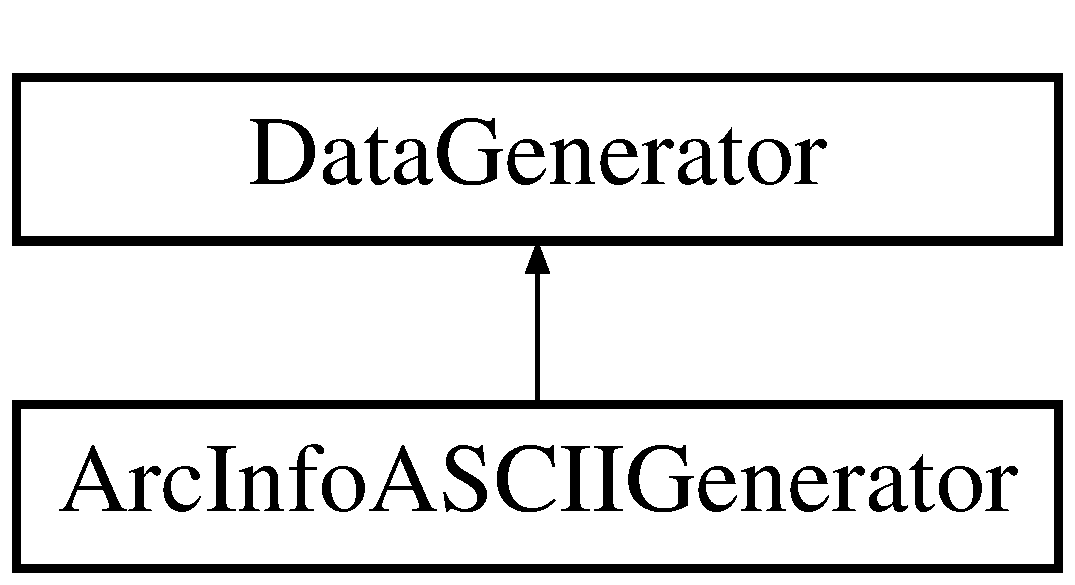
\includegraphics[height=2.000000cm]{classArcInfoASCIIGenerator}
\end{center}
\end{figure}
\subsection*{\-Classes}
\begin{DoxyCompactItemize}
\item 
struct \hyperlink{structArcInfoASCIIGenerator_1_1FileHeader}{\-File\-Header}
\begin{DoxyCompactList}\small\item\em file header for \-Arc/\-Info \-A\-S\-C\-I\-I file format \end{DoxyCompactList}\end{DoxyCompactItemize}
\subsection*{\-Public \-Member \-Functions}
\begin{DoxyCompactItemize}
\item 
\hyperlink{classArcInfoASCIIGenerator_ab0c7642cbf52bf5e86a66da76922bd43}{\-Arc\-Info\-A\-S\-C\-I\-I\-Generator} (const string \&\-\_\-file\-Name, const string \&\-\_\-file\-Directory)
\begin{DoxyCompactList}\small\item\em default constructor. use defualt values for both inherited member variables and self-\/declared variables \end{DoxyCompactList}\item 
\hypertarget{classArcInfoASCIIGenerator_a7de403bda7b658d45b94124c77ab9cc9}{\hyperlink{classArcInfoASCIIGenerator_a7de403bda7b658d45b94124c77ab9cc9}{\-Arc\-Info\-A\-S\-C\-I\-I\-Generator} (const char $\ast$\-\_\-file\-Name, const char $\ast$\-\_\-file\-Directory)}\label{classArcInfoASCIIGenerator_a7de403bda7b658d45b94124c77ab9cc9}

\begin{DoxyCompactList}\small\item\em constructor used to reset inherited member variables \end{DoxyCompactList}\item 
\hypertarget{classArcInfoASCIIGenerator_af4c006ea239d4427b3ab1bcb86704bd0}{\hyperlink{classArcInfoASCIIGenerator_af4c006ea239d4427b3ab1bcb86704bd0}{\-Arc\-Info\-A\-S\-C\-I\-I\-Generator} (const string \&\-\_\-file\-Name, const string \&\-\_\-file\-Directory, int \-\_\-n\-Rows, int \-\_\-n\-Cols, double \-\_\-xll\-Corner, double \-\_\-yll\-Corner, double \-\_\-cell\-Size, int \-\_\-no\-Value)}\label{classArcInfoASCIIGenerator_af4c006ea239d4427b3ab1bcb86704bd0}

\begin{DoxyCompactList}\small\item\em constructor used to reset both inherit members and self-\/declared members \end{DoxyCompactList}\item 
\hypertarget{classArcInfoASCIIGenerator_ae1cb5e813f12493afa5e94a65827488b}{\hyperlink{classArcInfoASCIIGenerator_ae1cb5e813f12493afa5e94a65827488b}{\-Arc\-Info\-A\-S\-C\-I\-I\-Generator} (int \-\_\-n\-Rows, int \-\_\-n\-Cols, double \-\_\-xll\-Corner, double \-\_\-yll\-Corner, double \-\_\-cell\-Size, int \-\_\-no\-Value)}\label{classArcInfoASCIIGenerator_ae1cb5e813f12493afa5e94a65827488b}

\begin{DoxyCompactList}\small\item\em constructor initialize self-\/declared member variables \end{DoxyCompactList}\item 
\hypertarget{classArcInfoASCIIGenerator_a985454ab0740ddc4fd0fcb6bec7b6c05}{bool \hyperlink{classArcInfoASCIIGenerator_a985454ab0740ddc4fd0fcb6bec7b6c05}{generate} (double min\-Value, double max\-Value, double step, int num\-Of\-Decimals, double no\-Value\-Percent)}\label{classArcInfoASCIIGenerator_a985454ab0740ddc4fd0fcb6bec7b6c05}

\begin{DoxyCompactList}\small\item\em function as describe in \hyperlink{DataGenerator_8h}{\-Data\-Generator.\-h} file \end{DoxyCompactList}\item 
\hypertarget{classArcInfoASCIIGenerator_a658168a9ebabc01febd8f1feced60041}{void \hyperlink{classArcInfoASCIIGenerator_a658168a9ebabc01febd8f1feced60041}{set\-Header} (int nrows, int ncols, double xllcorner, double yllcorner, double cellsize, int novalue)}\label{classArcInfoASCIIGenerator_a658168a9ebabc01febd8f1feced60041}

\begin{DoxyCompactList}\small\item\em setter. overloaded member function used to set the \-Arc/\-Info \-A\-S\-C\-I\-I file header \end{DoxyCompactList}\item 
\hypertarget{classArcInfoASCIIGenerator_af26ec3aa74fb8ef2c6b9b023b9138d71}{void \hyperlink{classArcInfoASCIIGenerator_af26ec3aa74fb8ef2c6b9b023b9138d71}{set\-Header} (\hyperlink{structArcInfoASCIIGenerator_1_1FileHeader}{\-File\-Header} \&tmp)}\label{classArcInfoASCIIGenerator_af26ec3aa74fb8ef2c6b9b023b9138d71}

\begin{DoxyCompactList}\small\item\em setter. overloaded member function used to set the \-Arc/\-Info \-A\-S\-C\-I\-I file header \end{DoxyCompactList}\item 
\hypertarget{classArcInfoASCIIGenerator_a2e5512db74f473c929fe0a06de92902d}{\hyperlink{structArcInfoASCIIGenerator_1_1FileHeader}{\-File\-Header} \& \hyperlink{classArcInfoASCIIGenerator_a2e5512db74f473c929fe0a06de92902d}{get\-Header} ()}\label{classArcInfoASCIIGenerator_a2e5512db74f473c929fe0a06de92902d}

\begin{DoxyCompactList}\small\item\em getter. member function used to get the file header \end{DoxyCompactList}\end{DoxyCompactItemize}


\subsection{\-Detailed \-Description}
\hyperlink{classArcInfoASCIIGenerator}{\-Arc\-Info\-A\-S\-C\-I\-I\-Generator} is inherited from \hyperlink{classDataGenerator}{\-Data\-Generator}, responsible for generating \-A\-R\-C/\-I\-N\-F\-O \-A\-S\-C\-I\-I data file. 

\-This class implements \char`\"{}\-Data\-Generator\-::generate(...)\char`\"{} virtual function, also including some self-\/declared member functions for setting/getting format specific infomation. 

\subsection{\-Constructor \& \-Destructor \-Documentation}
\hypertarget{classArcInfoASCIIGenerator_ab0c7642cbf52bf5e86a66da76922bd43}{\index{\-Arc\-Info\-A\-S\-C\-I\-I\-Generator@{\-Arc\-Info\-A\-S\-C\-I\-I\-Generator}!\-Arc\-Info\-A\-S\-C\-I\-I\-Generator@{\-Arc\-Info\-A\-S\-C\-I\-I\-Generator}}
\index{\-Arc\-Info\-A\-S\-C\-I\-I\-Generator@{\-Arc\-Info\-A\-S\-C\-I\-I\-Generator}!ArcInfoASCIIGenerator@{\-Arc\-Info\-A\-S\-C\-I\-I\-Generator}}
\subsubsection[{\-Arc\-Info\-A\-S\-C\-I\-I\-Generator}]{\setlength{\rightskip}{0pt plus 5cm}{\bf \-Arc\-Info\-A\-S\-C\-I\-I\-Generator\-::\-Arc\-Info\-A\-S\-C\-I\-I\-Generator} (
\begin{DoxyParamCaption}
\item[{const string \&}]{\-\_\-file\-Name, }
\item[{const string \&}]{\-\_\-file\-Directory}
\end{DoxyParamCaption}
)\hspace{0.3cm}{\ttfamily  \mbox{[}inline\mbox{]}}}}\label{classArcInfoASCIIGenerator_ab0c7642cbf52bf5e86a66da76922bd43}


default constructor. use defualt values for both inherited member variables and self-\/declared variables 

constructor used to reset inherited member variables from \hyperlink{classDataGenerator}{\-Data\-Generator} 

\-The documentation for this class was generated from the following files\-:\begin{DoxyCompactItemize}
\item 
include/\hyperlink{ArcInfoASCIIGenerator_8h}{\-Arc\-Info\-A\-S\-C\-I\-I\-Generator.\-h}\item 
src/\-Arc\-Info\-A\-S\-C\-I\-I\-Generator.\-cpp\end{DoxyCompactItemize}

\hypertarget{classArcInfoASCIIParser}{\section{\-Arc\-Info\-A\-S\-C\-I\-I\-Parser \-Class \-Reference}
\label{classArcInfoASCIIParser}\index{\-Arc\-Info\-A\-S\-C\-I\-I\-Parser@{\-Arc\-Info\-A\-S\-C\-I\-I\-Parser}}
}


class \hyperlink{classArcInfoASCIIParser}{\-Arc\-Info\-A\-S\-C\-I\-I\-Parser} is only used to parse \-Arc/\-Info \-A\-S\-C\-I\-I data file  




{\ttfamily \#include $<$\-Arc\-Info\-A\-S\-C\-I\-I\-Parser.\-h$>$}

\-Inheritance diagram for \-Arc\-Info\-A\-S\-C\-I\-I\-Parser\-:\begin{figure}[H]
\begin{center}
\leavevmode
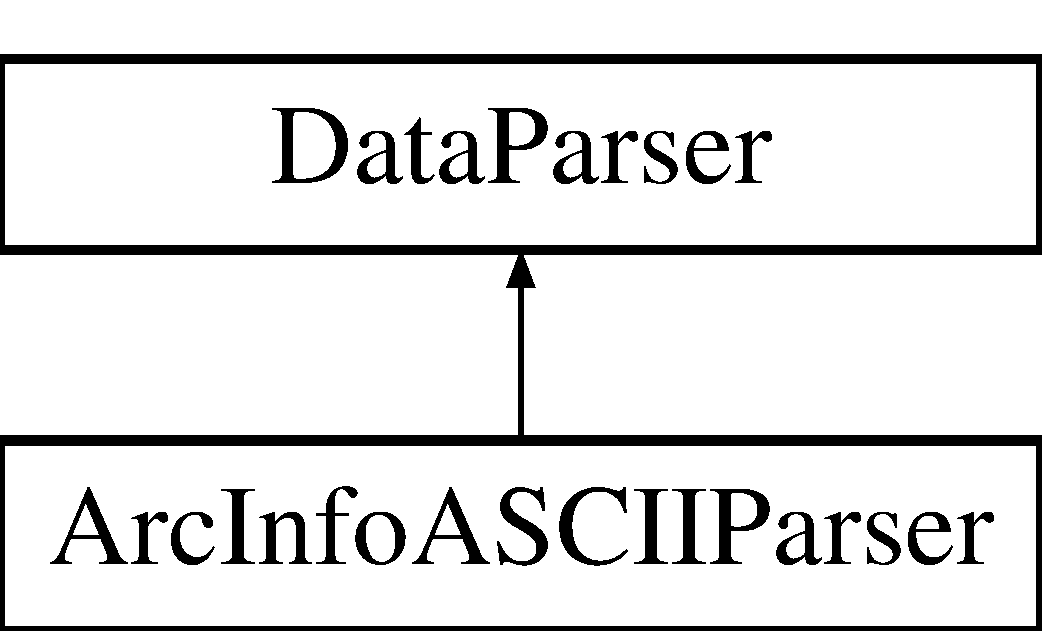
\includegraphics[height=2.000000cm]{classArcInfoASCIIParser}
\end{center}
\end{figure}
\subsection*{\-Public \-Member \-Functions}
\begin{DoxyCompactItemize}
\item 
\hypertarget{classArcInfoASCIIParser_a16289b738375476ff81fb802a5c470ee}{\hyperlink{classArcInfoASCIIParser_a16289b738375476ff81fb802a5c470ee}{\-Arc\-Info\-A\-S\-C\-I\-I\-Parser} ()}\label{classArcInfoASCIIParser_a16289b738375476ff81fb802a5c470ee}

\begin{DoxyCompactList}\small\item\em default constructor \end{DoxyCompactList}\item 
\hypertarget{classArcInfoASCIIParser_ae7ff0d38d9c1603fbecc49749dd4d31b}{\hyperlink{classArcInfoASCIIParser_ae7ff0d38d9c1603fbecc49749dd4d31b}{\-Arc\-Info\-A\-S\-C\-I\-I\-Parser} (const string \&\-\_\-file\-Path)}\label{classArcInfoASCIIParser_ae7ff0d38d9c1603fbecc49749dd4d31b}

\begin{DoxyCompactList}\small\item\em constructor set the filepath \end{DoxyCompactList}\item 
\hypertarget{classArcInfoASCIIParser_abe97d197a44d14edae52546d48079e1d}{\hyperlink{classArcInfoASCIIParser_abe97d197a44d14edae52546d48079e1d}{\-Arc\-Info\-A\-S\-C\-I\-I\-Parser} (const char $\ast$\-\_\-file\-Path)}\label{classArcInfoASCIIParser_abe97d197a44d14edae52546d48079e1d}

\begin{DoxyCompactList}\small\item\em constructor set the filepath \end{DoxyCompactList}\item 
\hypertarget{classArcInfoASCIIParser_a0f12fe096ddf4d7fe1ab4f3287a74b8b}{\hyperlink{classArcInfoASCIIParser_a0f12fe096ddf4d7fe1ab4f3287a74b8b}{$\sim$\-Arc\-Info\-A\-S\-C\-I\-I\-Parser} ()}\label{classArcInfoASCIIParser_a0f12fe096ddf4d7fe1ab4f3287a74b8b}

\begin{DoxyCompactList}\small\item\em destructor \end{DoxyCompactList}\item 
bool \hyperlink{classArcInfoASCIIParser_a1f63530762118826b85565479c98502a}{parse} (\hyperlink{classGridLayer}{\-Grid\-Layer} \&gl, int multiplier=1)
\begin{DoxyCompactList}\small\item\em pure virtual member function used to parse data into a int-\/valued grirdlayer \end{DoxyCompactList}\end{DoxyCompactItemize}


\subsection{\-Detailed \-Description}
class \hyperlink{classArcInfoASCIIParser}{\-Arc\-Info\-A\-S\-C\-I\-I\-Parser} is only used to parse \-Arc/\-Info \-A\-S\-C\-I\-I data file 

\subsection{\-Member \-Function \-Documentation}
\hypertarget{classArcInfoASCIIParser_a1f63530762118826b85565479c98502a}{\index{\-Arc\-Info\-A\-S\-C\-I\-I\-Parser@{\-Arc\-Info\-A\-S\-C\-I\-I\-Parser}!parse@{parse}}
\index{parse@{parse}!ArcInfoASCIIParser@{\-Arc\-Info\-A\-S\-C\-I\-I\-Parser}}
\subsubsection[{parse}]{\setlength{\rightskip}{0pt plus 5cm}bool {\bf \-Arc\-Info\-A\-S\-C\-I\-I\-Parser\-::parse} (
\begin{DoxyParamCaption}
\item[{{\bf \-Grid\-Layer} \&}]{gl, }
\item[{int}]{multiplier = {\ttfamily 1}}
\end{DoxyParamCaption}
)\hspace{0.3cm}{\ttfamily  \mbox{[}virtual\mbox{]}}}}\label{classArcInfoASCIIParser_a1f63530762118826b85565479c98502a}


pure virtual member function used to parse data into a int-\/valued grirdlayer 


\begin{DoxyParams}{\-Parameters}
{\em file\-Path} & the file path in disk \\
\hline
{\em gl} & the integer-\/valued grid layer to extract data to \\
\hline
{\em multiplier} & sometime all data in data file are small double, say 0.\-0032, the user can designate a multiplier, say 10000, then all data in grid layer will be multiplied by this multiplier, default to 1 \\
\hline
\end{DoxyParams}
\begin{DoxyReturn}{\-Returns}
true means successful, otherwise failed 
\end{DoxyReturn}


\-Implements \hyperlink{classDataParser_a45e498627eec0fc8638a34eab2ff2812}{\-Data\-Parser}.



\-The documentation for this class was generated from the following files\-:\begin{DoxyCompactItemize}
\item 
include/\hyperlink{ArcInfoASCIIParser_8h}{\-Arc\-Info\-A\-S\-C\-I\-I\-Parser.\-h}\item 
src/\-Arc\-Info\-A\-S\-C\-I\-I\-Parser.\-cpp\end{DoxyCompactItemize}

\hypertarget{classBlock}{\section{\-Block \-Class \-Reference}
\label{classBlock}\index{\-Block@{\-Block}}
}


class \char`\"{}\-Block\char`\"{} is specific for our project  




{\ttfamily \#include $<$\-Block.\-h$>$}

\-Inheritance diagram for \-Block\-:\begin{figure}[H]
\begin{center}
\leavevmode
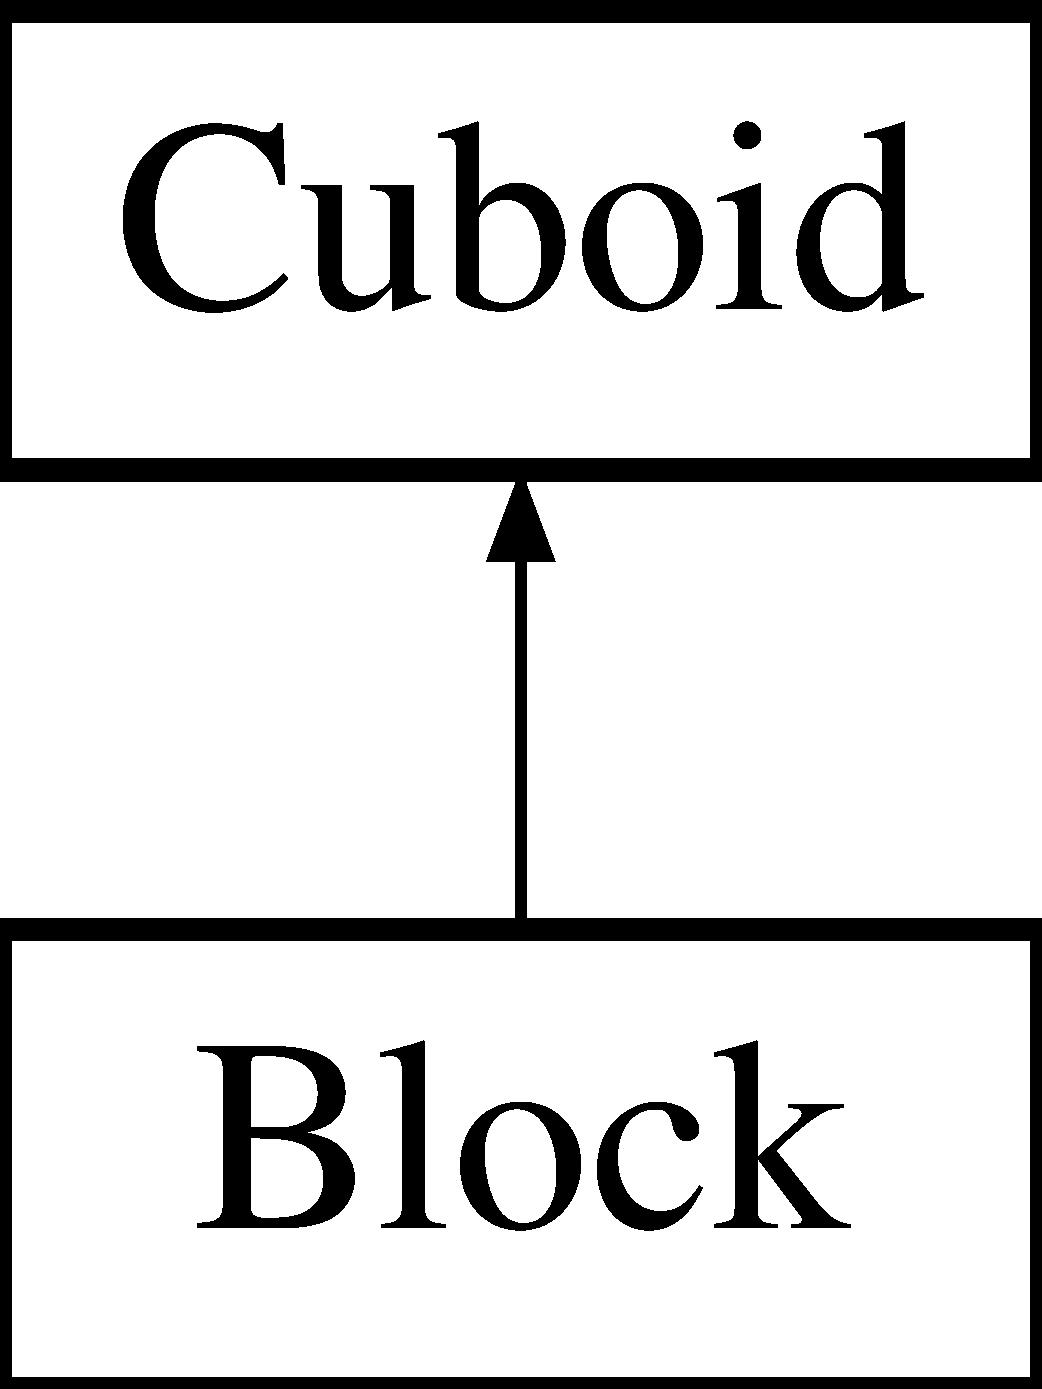
\includegraphics[height=2.000000cm]{classBlock}
\end{center}
\end{figure}
\subsection*{\-Public \-Member \-Functions}
\begin{DoxyCompactItemize}
\item 
\hypertarget{classBlock_a37658a946bf5067ad01d68d9ff086adc}{\hyperlink{classBlock_a37658a946bf5067ad01d68d9ff086adc}{\-Block} ()}\label{classBlock_a37658a946bf5067ad01d68d9ff086adc}

\begin{DoxyCompactList}\small\item\em default constructor \end{DoxyCompactList}\item 
\hypertarget{classBlock_a9be88ea094e64d4e8cf293554fba92f6}{\hyperlink{classBlock_a9be88ea094e64d4e8cf293554fba92f6}{\-Block} (int \-\_\-row\-Index, int \-\_\-column\-Index, int \-\_\-lower\-Layer\-Index, int \-\_\-upper\-Layer\-Index)}\label{classBlock_a9be88ea094e64d4e8cf293554fba92f6}

\begin{DoxyCompactList}\small\item\em constructor set indexing information for this block \end{DoxyCompactList}\item 
\hypertarget{classBlock_a225498988afa0931232800e67905c57e}{\hyperlink{classBlock_a225498988afa0931232800e67905c57e}{\-Block} (double \-\_\-longitude, double \-\_\-latitude, double \-\_\-length, \-Metric \-\_\-length\-Metric, double \-\_\-width, \-Metric \-\_\-width\-Metric, double \-\_\-height, \-Metric \-\_\-height\-Metric, double \-\_\-ground\-To\-Lower\-Base, int \-\_\-row\-Index, int \-\_\-column\-Index, int \-\_\-lower\-Layer\-Index, int \-\_\-upper\-Layer\-Index)}\label{classBlock_a225498988afa0931232800e67905c57e}

\begin{DoxyCompactList}\small\item\em constructor set some real geometric information and indexing information for the block \end{DoxyCompactList}\item 
\hypertarget{classBlock_aa89686c705375aae3dc8d8adb7cd9b0b}{int \hyperlink{classBlock_aa89686c705375aae3dc8d8adb7cd9b0b}{get\-Row\-Index} ()}\label{classBlock_aa89686c705375aae3dc8d8adb7cd9b0b}

\begin{DoxyCompactList}\small\item\em $>$ getter. get the row index of the block \end{DoxyCompactList}\item 
\hypertarget{classBlock_ac210bace38ac9f0396ad98ebdce28819}{int \hyperlink{classBlock_ac210bace38ac9f0396ad98ebdce28819}{get\-Column\-Index} ()}\label{classBlock_ac210bace38ac9f0396ad98ebdce28819}

\begin{DoxyCompactList}\small\item\em $>$ getter. get the column index of the block \end{DoxyCompactList}\item 
\hypertarget{classBlock_a2e1b3d6d31cd7aba4576a74524b6008c}{int \hyperlink{classBlock_a2e1b3d6d31cd7aba4576a74524b6008c}{get\-Lower\-Layer\-Index} ()}\label{classBlock_a2e1b3d6d31cd7aba4576a74524b6008c}

\begin{DoxyCompactList}\small\item\em $>$ getter. get the lower layer index \end{DoxyCompactList}\item 
\hypertarget{classBlock_a478e5c8832f9d89b7691f139c90c409c}{int \hyperlink{classBlock_a478e5c8832f9d89b7691f139c90c409c}{get\-Upper\-Layer\-Index} ()}\label{classBlock_a478e5c8832f9d89b7691f139c90c409c}

\begin{DoxyCompactList}\small\item\em $>$ getter. get the upper layer index \end{DoxyCompactList}\item 
\hypertarget{classBlock_a53c43ce4c0dfb5b21df780221f6e3515}{double \hyperlink{classBlock_a53c43ce4c0dfb5b21df780221f6e3515}{get\-Single\-Part\-Height} ()}\label{classBlock_a53c43ce4c0dfb5b21df780221f6e3515}

\begin{DoxyCompactList}\small\item\em $>$ getter. get the single length used by this block \end{DoxyCompactList}\item 
\hypertarget{classBlock_a84a48a65e4fa30689ed86b55fd5719d1}{long long \hyperlink{classBlock_a84a48a65e4fa30689ed86b55fd5719d1}{get\-Value} ()}\label{classBlock_a84a48a65e4fa30689ed86b55fd5719d1}

\begin{DoxyCompactList}\small\item\em $>$ getter. get the value store in this block \end{DoxyCompactList}\item 
\hypertarget{classBlock_aca5dc7b45373d87734ac76205449def5}{int \hyperlink{classBlock_aca5dc7b45373d87734ac76205449def5}{get\-Multiplier} ()}\label{classBlock_aca5dc7b45373d87734ac76205449def5}

\begin{DoxyCompactList}\small\item\em $>$ getter. get the \char`\"{}multiplier\char`\"{} used by \char`\"{}value\char`\"{} \end{DoxyCompactList}\item 
\hypertarget{classBlock_a0fe6984afe770ad046e0ffbe33398187}{void \hyperlink{classBlock_a0fe6984afe770ad046e0ffbe33398187}{set\-Row\-Index} (int \-\_\-row\-Index)}\label{classBlock_a0fe6984afe770ad046e0ffbe33398187}

\begin{DoxyCompactList}\small\item\em $>$ setter. set the row index of the block, seldom used, included here just for completeness \end{DoxyCompactList}\item 
\hypertarget{classBlock_aa7baf345a2178c30b77b2e4c92f2bd87}{void \hyperlink{classBlock_aa7baf345a2178c30b77b2e4c92f2bd87}{set\-Column\-Index} (int \-\_\-column\-Index)}\label{classBlock_aa7baf345a2178c30b77b2e4c92f2bd87}

\begin{DoxyCompactList}\small\item\em $>$ setter. set the column index of the block, seldom used, included here just for completeness \end{DoxyCompactList}\item 
\hypertarget{classBlock_a8c2e66acf65d4621369e68764bd16878}{void \hyperlink{classBlock_a8c2e66acf65d4621369e68764bd16878}{set\-Lower\-Layer\-Index} (int \-\_\-lower\-Layer\-Index)}\label{classBlock_a8c2e66acf65d4621369e68764bd16878}

\begin{DoxyCompactList}\small\item\em $>$ setter. set the lower layer index of the block, seldom used, included here just for completeness \end{DoxyCompactList}\item 
\hypertarget{classBlock_a0acbd3f89758131aa40fe0fa534f0bf8}{void \hyperlink{classBlock_a0acbd3f89758131aa40fe0fa534f0bf8}{set\-Upper\-Layer\-Index} (int \-\_\-upper\-Layer\-Index)}\label{classBlock_a0acbd3f89758131aa40fe0fa534f0bf8}

\begin{DoxyCompactList}\small\item\em $>$ setter. set the upper layer index of the block, seldom used, included here just for completeness \end{DoxyCompactList}\item 
\hypertarget{classBlock_a54819ef3e2f9c5e5529459b8cc100ebf}{void \hyperlink{classBlock_a54819ef3e2f9c5e5529459b8cc100ebf}{set\-Single\-Part\-Height} (double \-\_\-single\-Part\-Height)}\label{classBlock_a54819ef3e2f9c5e5529459b8cc100ebf}

\begin{DoxyCompactList}\small\item\em $>$ setter. set the single length used by this block. \end{DoxyCompactList}\item 
\hypertarget{classBlock_a0dbbe029ff3a2b1eba2bf2c72c6e24f8}{void \hyperlink{classBlock_a0dbbe029ff3a2b1eba2bf2c72c6e24f8}{set\-Value} (long long \-\_\-value)}\label{classBlock_a0dbbe029ff3a2b1eba2bf2c72c6e24f8}

\begin{DoxyCompactList}\small\item\em $>$ setter. set the value stores in block \end{DoxyCompactList}\item 
\hypertarget{classBlock_a96cc83144bdea419727df03687a1be63}{void \hyperlink{classBlock_a96cc83144bdea419727df03687a1be63}{set\-Multiplier} (int \-\_\-multiplier)}\label{classBlock_a96cc83144bdea419727df03687a1be63}

\begin{DoxyCompactList}\small\item\em $>$ setter. set the \char`\"{}multiplier\char`\"{} used by \char`\"{}value\char`\"{} \end{DoxyCompactList}\end{DoxyCompactItemize}


\subsection{\-Detailed \-Description}
class \char`\"{}\-Block\char`\"{} is specific for our project 

class \char`\"{}\-Block\char`\"{} on one hand have all properties inherit from \char`\"{}\-Cuboid\char`\"{}, the meanings of member variables are the same with in \char`\"{}\-Cuboid\char`\"{}, on the other hand, for our project, \char`\"{}\-Block\char`\"{} should have some other info to record its position after interpolating the \char`\"{}\-Grid\-Layer\char`\"{}, so we will add \char`\"{}indexing\char`\"{} properties to \char`\"{}\-Block\char`\"{} 

\-The documentation for this class was generated from the following files\-:\begin{DoxyCompactItemize}
\item 
include/\hyperlink{Block_8h}{\-Block.\-h}\item 
src/\hyperlink{Block_8cpp}{\-Block.\-cpp}\end{DoxyCompactItemize}

\hypertarget{classCuboid}{\section{\-Cuboid \-Class \-Reference}
\label{classCuboid}\index{\-Cuboid@{\-Cuboid}}
}


class \char`\"{}\-Cuboid\char`\"{} is a cuboid which exist in 3\-D geometric space  




{\ttfamily \#include $<$\-Cuboid.\-h$>$}

\-Inheritance diagram for \-Cuboid\-:\begin{figure}[H]
\begin{center}
\leavevmode
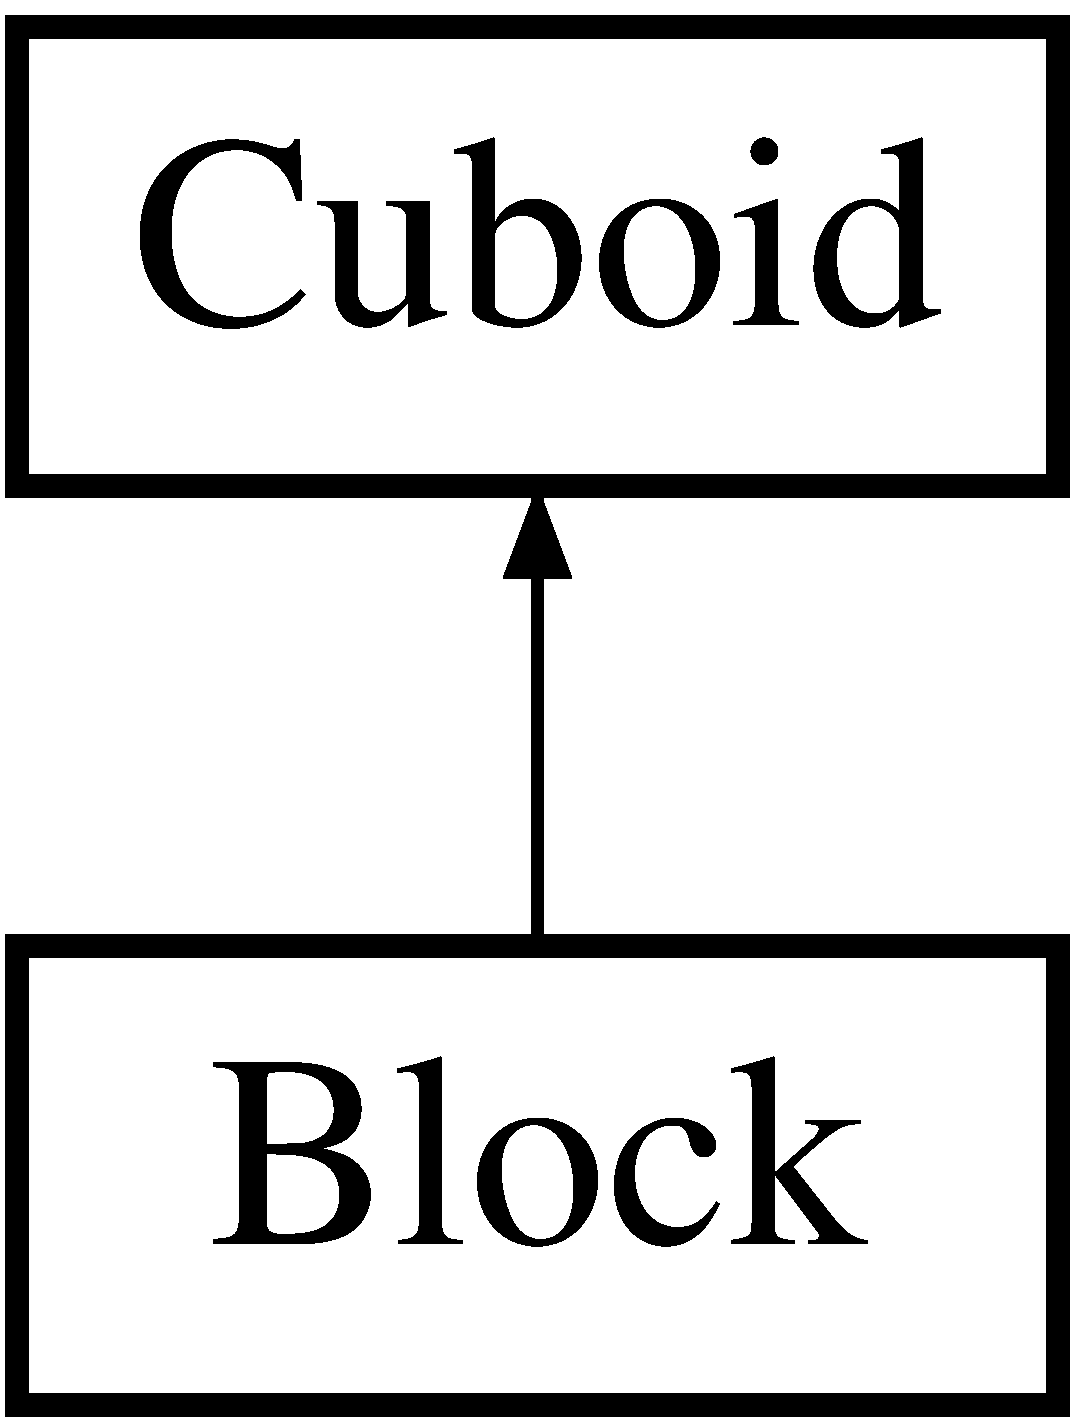
\includegraphics[height=2.000000cm]{classCuboid}
\end{center}
\end{figure}
\subsection*{\-Public \-Member \-Functions}
\begin{DoxyCompactItemize}
\item 
\hypertarget{classCuboid_a0035f798f5284b6af5f25ed88cb216e8}{{\bfseries \-Cuboid} (double \-\_\-longitude, double \-\_\-latitude, double \-\_\-length, \-Metric \-\_\-length\-Metric, double \-\_\-width, \-Metric \-\_\-width\-Metric, double \-\_\-height, \-Metric \-\_\-height\-Metric, double \-\_\-ground\-To\-Lower\-Base)}\label{classCuboid_a0035f798f5284b6af5f25ed88cb216e8}

\item 
\hypertarget{classCuboid_aa2bd1dcbfd72948c2396f379bc2343c0}{{\bfseries \-Cuboid} (double \-\_\-longitude, double \-\_\-latitude, double \-\_\-length, double \-\_\-width, double \-\_\-height, double \-\_\-ground\-To\-Lower\-Base)}\label{classCuboid_aa2bd1dcbfd72948c2396f379bc2343c0}

\item 
\hypertarget{classCuboid_a7e020aa4d4a3f4a18fb66f5508a37e7c}{double \hyperlink{classCuboid_a7e020aa4d4a3f4a18fb66f5508a37e7c}{get\-Longitude} ()}\label{classCuboid_a7e020aa4d4a3f4a18fb66f5508a37e7c}

\begin{DoxyCompactList}\small\item\em $>$ getter. get the longitude of the bounding cuboid \end{DoxyCompactList}\item 
\hypertarget{classCuboid_a4a64680a0f69c85bd5d973665e974d45}{double \hyperlink{classCuboid_a4a64680a0f69c85bd5d973665e974d45}{get\-Latitude} ()}\label{classCuboid_a4a64680a0f69c85bd5d973665e974d45}

\begin{DoxyCompactList}\small\item\em $>$ getter. get the latitude of the bounding cuboid \end{DoxyCompactList}\item 
\hypertarget{classCuboid_a2ba0dd1e23699927d1e3f3d0189d2f33}{double \hyperlink{classCuboid_a2ba0dd1e23699927d1e3f3d0189d2f33}{get\-Length} ()}\label{classCuboid_a2ba0dd1e23699927d1e3f3d0189d2f33}

\begin{DoxyCompactList}\small\item\em $>$ getter. get the length of the bounding cuboid \end{DoxyCompactList}\item 
\hypertarget{classCuboid_a105cff168c3775658a9e4fb02a69d2a5}{\-Metric \hyperlink{classCuboid_a105cff168c3775658a9e4fb02a69d2a5}{get\-Length\-Metric} ()}\label{classCuboid_a105cff168c3775658a9e4fb02a69d2a5}

\begin{DoxyCompactList}\small\item\em $>$ getter. get the metric used by length \end{DoxyCompactList}\item 
\hypertarget{classCuboid_a2609713a4da6a9fbaabdb7188379dbd1}{double \hyperlink{classCuboid_a2609713a4da6a9fbaabdb7188379dbd1}{get\-Width} ()}\label{classCuboid_a2609713a4da6a9fbaabdb7188379dbd1}

\begin{DoxyCompactList}\small\item\em $>$ getter. get the width of the bounding cuboid \end{DoxyCompactList}\item 
\hypertarget{classCuboid_a008ee0b1d50806842860cb3eed3d0edb}{\-Metric \hyperlink{classCuboid_a008ee0b1d50806842860cb3eed3d0edb}{get\-Width\-Metric} ()}\label{classCuboid_a008ee0b1d50806842860cb3eed3d0edb}

\begin{DoxyCompactList}\small\item\em $>$ getter. get the metric used by width \end{DoxyCompactList}\item 
\hypertarget{classCuboid_a5bb8679b9237b122f1120a185b6bc0c6}{double \hyperlink{classCuboid_a5bb8679b9237b122f1120a185b6bc0c6}{get\-Height} ()}\label{classCuboid_a5bb8679b9237b122f1120a185b6bc0c6}

\begin{DoxyCompactList}\small\item\em $>$ getter. get the height of the bounding cuboid \end{DoxyCompactList}\item 
\hypertarget{classCuboid_a73fa2a69870dac37de851937d5fd3144}{\-Metric \hyperlink{classCuboid_a73fa2a69870dac37de851937d5fd3144}{get\-Height\-Metric} ()}\label{classCuboid_a73fa2a69870dac37de851937d5fd3144}

\begin{DoxyCompactList}\small\item\em $>$ getter. get the metric used by height \end{DoxyCompactList}\item 
\hypertarget{classCuboid_a91c029028720a94825bed667d86dc959}{double \hyperlink{classCuboid_a91c029028720a94825bed667d86dc959}{get\-Ground\-To\-Lower\-Base} ()}\label{classCuboid_a91c029028720a94825bed667d86dc959}

\begin{DoxyCompactList}\small\item\em $>$ getter. get the vertical distance from ground to lower base \end{DoxyCompactList}\item 
\hypertarget{classCuboid_ac5ead5e6e2b5e9a18d7ca5990b38b3e4}{void \hyperlink{classCuboid_ac5ead5e6e2b5e9a18d7ca5990b38b3e4}{set\-Longitude} (double \-\_\-longitude)}\label{classCuboid_ac5ead5e6e2b5e9a18d7ca5990b38b3e4}

\begin{DoxyCompactList}\small\item\em $>$ setter. set the longitude of the bounding cuboid \end{DoxyCompactList}\item 
\hypertarget{classCuboid_a723c412d9beb6e6e4cba2d743fb62f2a}{void \hyperlink{classCuboid_a723c412d9beb6e6e4cba2d743fb62f2a}{set\-Latitude} (double \-\_\-latitude)}\label{classCuboid_a723c412d9beb6e6e4cba2d743fb62f2a}

\begin{DoxyCompactList}\small\item\em $>$ setter. set the latitude of the bounding cuboid \end{DoxyCompactList}\item 
\hypertarget{classCuboid_afd2a9a5c2037b7f741301893436c5c95}{void \hyperlink{classCuboid_afd2a9a5c2037b7f741301893436c5c95}{set\-Length} (double \-\_\-length)}\label{classCuboid_afd2a9a5c2037b7f741301893436c5c95}

\begin{DoxyCompactList}\small\item\em $>$ setter. set the length of the bounding cuboid \end{DoxyCompactList}\item 
\hypertarget{classCuboid_a95e113f2dc9d6bfc7c40882e2461d737}{void \hyperlink{classCuboid_a95e113f2dc9d6bfc7c40882e2461d737}{set\-Length\-Metric} (\-Metric \-\_\-length\-Metric)}\label{classCuboid_a95e113f2dc9d6bfc7c40882e2461d737}

\begin{DoxyCompactList}\small\item\em $>$ setter. set the metric used by \char`\"{}length\char`\"{} \end{DoxyCompactList}\item 
\hypertarget{classCuboid_a46efc5a1a0ad31c8e40269c10837a394}{void \hyperlink{classCuboid_a46efc5a1a0ad31c8e40269c10837a394}{set\-Width} (double \-\_\-width)}\label{classCuboid_a46efc5a1a0ad31c8e40269c10837a394}

\begin{DoxyCompactList}\small\item\em $>$ setter. set the width of the bounding cuboid \end{DoxyCompactList}\item 
\hypertarget{classCuboid_ac63f89feef84839069d5708f51bda9c3}{void \hyperlink{classCuboid_ac63f89feef84839069d5708f51bda9c3}{set\-Width\-Metric} (\-Metric \-\_\-widht\-Metric)}\label{classCuboid_ac63f89feef84839069d5708f51bda9c3}

\begin{DoxyCompactList}\small\item\em $>$ setter. set the metric used by \char`\"{}width\char`\"{} \end{DoxyCompactList}\item 
\hypertarget{classCuboid_a2bb58d4f8399ac1bff23edde5648a827}{void \hyperlink{classCuboid_a2bb58d4f8399ac1bff23edde5648a827}{set\-Height} (double \-\_\-height)}\label{classCuboid_a2bb58d4f8399ac1bff23edde5648a827}

\begin{DoxyCompactList}\small\item\em $>$ setter. set the height of the cuboid \end{DoxyCompactList}\item 
\hypertarget{classCuboid_a1eb75213e981310ea10f153da2b21a5f}{void \hyperlink{classCuboid_a1eb75213e981310ea10f153da2b21a5f}{set\-Height\-Metric} (\-Metric \-\_\-height\-Metric)}\label{classCuboid_a1eb75213e981310ea10f153da2b21a5f}

\begin{DoxyCompactList}\small\item\em $>$ setter. set the metric used by \char`\"{}height\char`\"{} \end{DoxyCompactList}\item 
\hypertarget{classCuboid_a77e5163fee5733c735acc57b6e9cc9f5}{void \hyperlink{classCuboid_a77e5163fee5733c735acc57b6e9cc9f5}{set\-Ground\-To\-Lower\-Base} (double \-\_\-ground\-To\-Lower\-Base)}\label{classCuboid_a77e5163fee5733c735acc57b6e9cc9f5}

\begin{DoxyCompactList}\small\item\em $>$ setter. set the ground to lower base distance \end{DoxyCompactList}\item 
\hypertarget{classCuboid_a34979a3e201b3a2131039702ae4120cc}{double \hyperlink{classCuboid_a34979a3e201b3a2131039702ae4120cc}{get\-Base\-Area\-Size} (const \-Metric \&metric)}\label{classCuboid_a34979a3e201b3a2131039702ae4120cc}

\begin{DoxyCompactList}\small\item\em $>$ get the area of the base. parameter metric designate the metric used when calculating \end{DoxyCompactList}\item 
\hypertarget{classCuboid_a10d733aa5ce514deac6ee0fca510695c}{double \hyperlink{classCuboid_a10d733aa5ce514deac6ee0fca510695c}{get\-Shell\-Area\-Size} (const \-Metric \&metric)}\label{classCuboid_a10d733aa5ce514deac6ee0fca510695c}

\begin{DoxyCompactList}\small\item\em $>$ get the shell area size \end{DoxyCompactList}\item 
\hypertarget{classCuboid_a814655a4dad4ddc9e2e743a19786088e}{double \hyperlink{classCuboid_a814655a4dad4ddc9e2e743a19786088e}{get\-Volume\-Size} (const \-Metric \&metric)}\label{classCuboid_a814655a4dad4ddc9e2e743a19786088e}

\begin{DoxyCompactList}\small\item\em $>$ get the cuboid's volume size \end{DoxyCompactList}\end{DoxyCompactItemize}
\subsection*{\-Protected \-Attributes}
\begin{DoxyCompactItemize}
\item 
\hypertarget{classCuboid_aca08c9b1c33c722ddfd46405b568ba65}{double \hyperlink{classCuboid_aca08c9b1c33c722ddfd46405b568ba65}{longitude}}\label{classCuboid_aca08c9b1c33c722ddfd46405b568ba65}

\begin{DoxyCompactList}\small\item\em $>$ longitude of southwest point of the lower base \end{DoxyCompactList}\item 
\hypertarget{classCuboid_aec4c8b92658c731e2b8745e6b2418375}{double \hyperlink{classCuboid_aec4c8b92658c731e2b8745e6b2418375}{latitude}}\label{classCuboid_aec4c8b92658c731e2b8745e6b2418375}

\begin{DoxyCompactList}\small\item\em $>$ latitude of southwest point of the lower base \end{DoxyCompactList}\item 
\hypertarget{classCuboid_ae1fa9e6e59887437842de9fdc9cdc13b}{double \hyperlink{classCuboid_ae1fa9e6e59887437842de9fdc9cdc13b}{length}}\label{classCuboid_ae1fa9e6e59887437842de9fdc9cdc13b}

\begin{DoxyCompactList}\small\item\em $>$ distance from west to east \end{DoxyCompactList}\item 
\hypertarget{classCuboid_a979bb7b92b101cfac63780b705c280c4}{\-Metric \hyperlink{classCuboid_a979bb7b92b101cfac63780b705c280c4}{length\-Metric}}\label{classCuboid_a979bb7b92b101cfac63780b705c280c4}

\begin{DoxyCompactList}\small\item\em $>$ metric used by \char`\"{}length\char`\"{} \end{DoxyCompactList}\item 
\hypertarget{classCuboid_a441591b764c8afbf763c77f28a9903b7}{double \hyperlink{classCuboid_a441591b764c8afbf763c77f28a9903b7}{width}}\label{classCuboid_a441591b764c8afbf763c77f28a9903b7}

\begin{DoxyCompactList}\small\item\em $>$ distance from north to south \end{DoxyCompactList}\item 
\hypertarget{classCuboid_a12b3c54f5ba533d55b6ff998dd2a341a}{\-Metric \hyperlink{classCuboid_a12b3c54f5ba533d55b6ff998dd2a341a}{width\-Metric}}\label{classCuboid_a12b3c54f5ba533d55b6ff998dd2a341a}

\begin{DoxyCompactList}\small\item\em $>$ metric used by \char`\"{}width\char`\"{} \end{DoxyCompactList}\item 
\hypertarget{classCuboid_aded3775fba282d4d1065cbf7cd20f569}{double \hyperlink{classCuboid_aded3775fba282d4d1065cbf7cd20f569}{height}}\label{classCuboid_aded3775fba282d4d1065cbf7cd20f569}

\begin{DoxyCompactList}\small\item\em $>$ vertical distance from lower base to upper base \end{DoxyCompactList}\item 
\hypertarget{classCuboid_a686ee4124225b3ccc6769104882f6672}{\-Metric \hyperlink{classCuboid_a686ee4124225b3ccc6769104882f6672}{height\-Metric}}\label{classCuboid_a686ee4124225b3ccc6769104882f6672}

\begin{DoxyCompactList}\small\item\em $>$ metric used by \char`\"{}height\char`\"{}, this metric is same with metric used by \char`\"{}ground\-To\-Lower\-Base\char`\"{} \end{DoxyCompactList}\item 
\hypertarget{classCuboid_afb9b133c1eb5f90fafbae84d4e4fe639}{double \hyperlink{classCuboid_afb9b133c1eb5f90fafbae84d4e4fe639}{ground\-To\-Lower\-Base}}\label{classCuboid_afb9b133c1eb5f90fafbae84d4e4fe639}

\begin{DoxyCompactList}\small\item\em $>$ vertical distance from earth surface to lower base \end{DoxyCompactList}\end{DoxyCompactItemize}


\subsection{\-Detailed \-Description}
class \char`\"{}\-Cuboid\char`\"{} is a cuboid which exist in 3\-D geometric space 

\-This class defines fundamental properties and functions of a \char`\"{}\-Cuboid\char`\"{}. \-These is an issue with function \char`\"{}set\-Length(...)\char`\"{}, \char`\"{}set\-Length\-Metric(...)\char`\"{}, should we combine these two as one function since these two are strongly related 

\-The documentation for this class was generated from the following files\-:\begin{DoxyCompactItemize}
\item 
include/\-Cuboid.\-h\item 
src/\-Cuboid.\-cpp\end{DoxyCompactItemize}

\hypertarget{classDataGenerator}{\section{\-Data\-Generator \-Class \-Reference}
\label{classDataGenerator}\index{\-Data\-Generator@{\-Data\-Generator}}
}


virtual class to define general properties for data generator  




{\ttfamily \#include $<$\-Data\-Generator.\-h$>$}

\-Inheritance diagram for \-Data\-Generator\-:\begin{figure}[H]
\begin{center}
\leavevmode
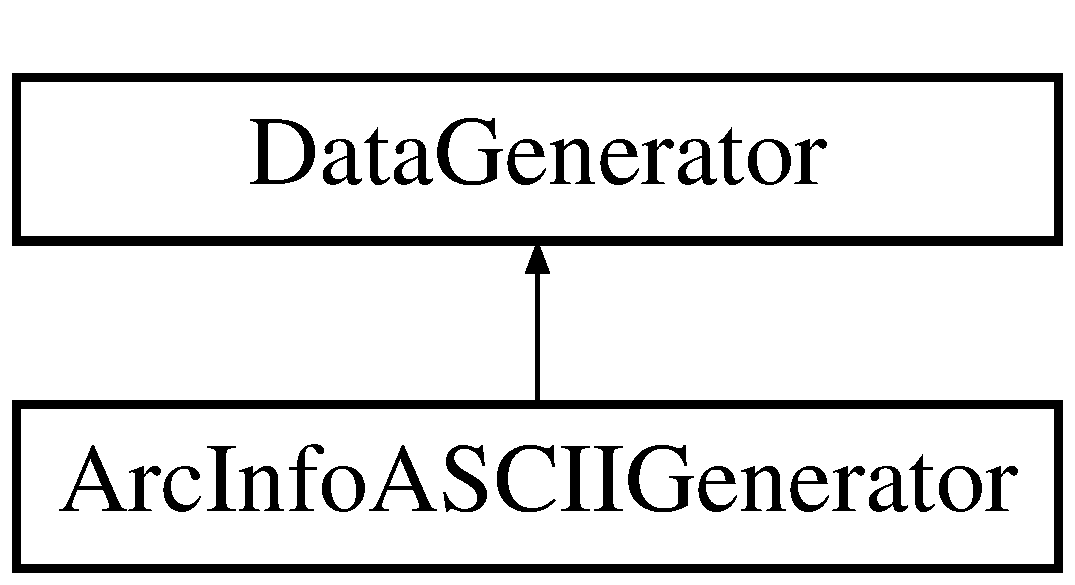
\includegraphics[height=2.000000cm]{classDataGenerator}
\end{center}
\end{figure}
\subsection*{\-Public \-Member \-Functions}
\begin{DoxyCompactItemize}
\item 
\hypertarget{classDataGenerator_a1b096a6b707523c5561a7961b5d635b1}{\hyperlink{classDataGenerator_a1b096a6b707523c5561a7961b5d635b1}{\-Data\-Generator} ()}\label{classDataGenerator_a1b096a6b707523c5561a7961b5d635b1}

\begin{DoxyCompactList}\small\item\em default constructor, put the generated data file in \char`\"{}currently directory\char`\"{}, file name to be \char`\"{}\-N\-O\-N\-S\-E\-N\-S\-E\char`\"{}, file type to be \char`\"{}\-N\-O\-N\-S\-E\-N\-S\-E\char`\"{} \end{DoxyCompactList}\item 
\hypertarget{classDataGenerator_a91666b97997fbb3ebfd5bd5da47ab07d}{\hyperlink{classDataGenerator_a91666b97997fbb3ebfd5bd5da47ab07d}{\-Data\-Generator} (const string \&\-\_\-file\-Name, const string \&\-\_\-file\-Directory, \hyperlink{FileType_8h_a2c794c5c13ab4dd7e65bad031dbe41c3}{\-File\-Type} \-\_\-file\-Type)}\label{classDataGenerator_a91666b97997fbb3ebfd5bd5da47ab07d}

\begin{DoxyCompactList}\small\item\em constructor utilize list initialization, accepts c++ string class as parameters type \end{DoxyCompactList}\item 
\hypertarget{classDataGenerator_a32248aac87220f988e50cf1aaee979f7}{\hyperlink{classDataGenerator_a32248aac87220f988e50cf1aaee979f7}{\-Data\-Generator} (\hyperlink{FileType_8h_a2c794c5c13ab4dd7e65bad031dbe41c3}{\-File\-Type} \-\_\-file\-Type)}\label{classDataGenerator_a32248aac87220f988e50cf1aaee979f7}

\begin{DoxyCompactList}\small\item\em constructor set file\-Type with other default \end{DoxyCompactList}\item 
\hypertarget{classDataGenerator_a7e007f23a4bc18126117a44a7f0982a7}{\hyperlink{classDataGenerator_a7e007f23a4bc18126117a44a7f0982a7}{\-Data\-Generator} (const char $\ast$\-\_\-file\-Name, const char $\ast$\-\_\-file\-Directory, \hyperlink{FileType_8h_a2c794c5c13ab4dd7e65bad031dbe41c3}{\-File\-Type} \-\_\-file\-Type)}\label{classDataGenerator_a7e007f23a4bc18126117a44a7f0982a7}

\begin{DoxyCompactList}\small\item\em constructor utilize list initialization, accepts c chars as parameters type \end{DoxyCompactList}\item 
\hypertarget{classDataGenerator_aa0efe82e850a32a8dc18fcbe99da6bf4}{virtual \hyperlink{classDataGenerator_aa0efe82e850a32a8dc18fcbe99da6bf4}{$\sim$\-Data\-Generator} ()}\label{classDataGenerator_aa0efe82e850a32a8dc18fcbe99da6bf4}

\begin{DoxyCompactList}\small\item\em pure virtual destructor \end{DoxyCompactList}\item 
\hypertarget{classDataGenerator_adb362b34246ae1567b304a970e1c84f8}{void \hyperlink{classDataGenerator_adb362b34246ae1567b304a970e1c84f8}{set\-File\-Name} (const string \&\-\_\-file\-Name)}\label{classDataGenerator_adb362b34246ae1567b304a970e1c84f8}

\begin{DoxyCompactList}\small\item\em setter. overloaded member function, set the generated data file name, accept c++ string class as parameter type \end{DoxyCompactList}\item 
\hypertarget{classDataGenerator_a3b36d96241705dd8c625c9a629ad7b3e}{void \hyperlink{classDataGenerator_a3b36d96241705dd8c625c9a629ad7b3e}{set\-File\-Name} (const char $\ast$\-\_\-file\-Name)}\label{classDataGenerator_a3b36d96241705dd8c625c9a629ad7b3e}

\begin{DoxyCompactList}\small\item\em setter. overloaded member function, set the generated data file name, accept c chars as parameter type \end{DoxyCompactList}\item 
\hypertarget{classDataGenerator_a08252e83067f3f635dafc43ef44a5d40}{void \hyperlink{classDataGenerator_a08252e83067f3f635dafc43ef44a5d40}{set\-File\-Directory} (const string \&\-\_\-file\-Directory)}\label{classDataGenerator_a08252e83067f3f635dafc43ef44a5d40}

\begin{DoxyCompactList}\small\item\em setter. overloaded member function, set the directory for the generated data file, accept string class as parameter type \end{DoxyCompactList}\item 
\hypertarget{classDataGenerator_a4a62575e04f21f18aad89327dffd6b6d}{void \hyperlink{classDataGenerator_a4a62575e04f21f18aad89327dffd6b6d}{set\-File\-Directory} (const char $\ast$\-\_\-file\-Directory)}\label{classDataGenerator_a4a62575e04f21f18aad89327dffd6b6d}

\begin{DoxyCompactList}\small\item\em setter. overloaded member function, set the directory for the generated data file, accept c chars as parameter type \end{DoxyCompactList}\item 
\hypertarget{classDataGenerator_af9b368a1ea6e6a0622c691d7ccadae12}{void \hyperlink{classDataGenerator_af9b368a1ea6e6a0622c691d7ccadae12}{set\-File\-Type} (\hyperlink{FileType_8h_a2c794c5c13ab4dd7e65bad031dbe41c3}{\-File\-Type} \-\_\-file\-Tyep)}\label{classDataGenerator_af9b368a1ea6e6a0622c691d7ccadae12}

\begin{DoxyCompactList}\small\item\em setter. set the file type \end{DoxyCompactList}\item 
\hypertarget{classDataGenerator_acae2a977b7525af309433978c8dee9de}{string \hyperlink{classDataGenerator_acae2a977b7525af309433978c8dee9de}{get\-File\-Name} ()}\label{classDataGenerator_acae2a977b7525af309433978c8dee9de}

\begin{DoxyCompactList}\small\item\em getter. get the generated data file name, including any prefix or postfix, not include directory \end{DoxyCompactList}\item 
\hypertarget{classDataGenerator_addc30af98e4f589ff9b1b04d03cbef9a}{string \hyperlink{classDataGenerator_addc30af98e4f589ff9b1b04d03cbef9a}{get\-File\-Directory} ()}\label{classDataGenerator_addc30af98e4f589ff9b1b04d03cbef9a}

\begin{DoxyCompactList}\small\item\em getter. get the file directory of the generated data file, always have char \char`\"{}/\char`\"{} as the last character \end{DoxyCompactList}\item 
\hypertarget{classDataGenerator_ab4505d83948a30240c83c42d42f79e01}{\hyperlink{FileType_8h_a2c794c5c13ab4dd7e65bad031dbe41c3}{\-File\-Type} \hyperlink{classDataGenerator_ab4505d83948a30240c83c42d42f79e01}{get\-File\-Type} ()}\label{classDataGenerator_ab4505d83948a30240c83c42d42f79e01}

\begin{DoxyCompactList}\small\item\em getter. get the file type for the generated data file, value should exist in \char`\"{}enum File\-Type\{...\}\char`\"{} \end{DoxyCompactList}\item 
virtual bool \hyperlink{classDataGenerator_a58deadd2230db351b03c85d2f8f0a5d6}{generate} (double min\-Value, double max\-Value, double step, int num\-Of\-Decimals, double no\-Value\-Percent)=0
\begin{DoxyCompactList}\small\item\em pure virtual member function responsible for generating data file \end{DoxyCompactList}\end{DoxyCompactItemize}
\subsection*{\-Protected \-Attributes}
\begin{DoxyCompactItemize}
\item 
\hypertarget{classDataGenerator_a4f4d384cfa418e73e3cb948968398e1a}{\hyperlink{FileType_8h_a2c794c5c13ab4dd7e65bad031dbe41c3}{\-File\-Type} \hyperlink{classDataGenerator_a4f4d384cfa418e73e3cb948968398e1a}{file\-Type}}\label{classDataGenerator_a4f4d384cfa418e73e3cb948968398e1a}

\begin{DoxyCompactList}\small\item\em denotes in which file format would the generated data file be \end{DoxyCompactList}\item 
\hypertarget{classDataGenerator_a0bfe4164d57ad70cdf91a63770bb5317}{string \hyperlink{classDataGenerator_a0bfe4164d57ad70cdf91a63770bb5317}{file\-Name}}\label{classDataGenerator_a0bfe4164d57ad70cdf91a63770bb5317}

\begin{DoxyCompactList}\small\item\em denotes the file name of the generated data file, any prefix or postfix included. \end{DoxyCompactList}\item 
\hypertarget{classDataGenerator_a4ed887b424833bb723d105983c61023d}{string \hyperlink{classDataGenerator_a4ed887b424833bb723d105983c61023d}{file\-Directory}}\label{classDataGenerator_a4ed887b424833bb723d105983c61023d}

\begin{DoxyCompactList}\small\item\em denotes the file directory of the generated data file. the last character should be exactly the character \char`\"{}/\char`\"{} \end{DoxyCompactList}\end{DoxyCompactItemize}


\subsection{\-Detailed \-Description}
virtual class to define general properties for data generator 

\-This class provides several constructors, several setters and getters for users to set/retrieve corresponding info associated with generated data file 

\subsection{\-Member \-Function \-Documentation}
\hypertarget{classDataGenerator_a58deadd2230db351b03c85d2f8f0a5d6}{\index{\-Data\-Generator@{\-Data\-Generator}!generate@{generate}}
\index{generate@{generate}!DataGenerator@{\-Data\-Generator}}
\subsubsection[{generate}]{\setlength{\rightskip}{0pt plus 5cm}virtual bool {\bf \-Data\-Generator\-::generate} (
\begin{DoxyParamCaption}
\item[{double}]{min\-Value, }
\item[{double}]{max\-Value, }
\item[{double}]{step, }
\item[{int}]{num\-Of\-Decimals, }
\item[{double}]{no\-Value\-Percent}
\end{DoxyParamCaption}
)\hspace{0.3cm}{\ttfamily  \mbox{[}pure virtual\mbox{]}}}}\label{classDataGenerator_a58deadd2230db351b03c85d2f8f0a5d6}


pure virtual member function responsible for generating data file 

\begin{DoxyReturn}{\-Returns}
true denotes generating data file successfully, false otherwise 
\end{DoxyReturn}

\begin{DoxyParams}{\-Parameters}
{\em min\-Value} & minimum numeric data in data file \\
\hline
{\em max\-Value} & maximum numeric data in data file \\
\hline
{\em step} & used to set numeric increment \\
\hline
{\em num\-Of\-Decimals} & indicate the number of digits in after decimal point, 0 means numeric data are all integers \\
\hline
{\em no\-Value\-Percent} & used to represent the percentage the null value should exist in a data file \\
\hline
\end{DoxyParams}


\-Implemented in \hyperlink{classArcInfoASCIIGenerator_a985454ab0740ddc4fd0fcb6bec7b6c05}{\-Arc\-Info\-A\-S\-C\-I\-I\-Generator}.



\-The documentation for this class was generated from the following files\-:\begin{DoxyCompactItemize}
\item 
include/\hyperlink{DataGenerator_8h}{\-Data\-Generator.\-h}\item 
src/\-Data\-Generator.\-cpp\end{DoxyCompactItemize}

\hypertarget{structDataInfo}{\section{\-Data\-Info \-Struct \-Reference}
\label{structDataInfo}\index{\-Data\-Info@{\-Data\-Info}}
}


data structure to keep some detailed information for the data in a data file  




{\ttfamily \#include $<$\-Grid\-Layer.\-h$>$}

\subsection*{\-Public \-Member \-Functions}
\begin{DoxyCompactItemize}
\item 
\hypertarget{structDataInfo_a1bf2df99d22b1b70f5ff75e9ea922159}{\hyperlink{structDataInfo_a1bf2df99d22b1b70f5ff75e9ea922159}{\-Data\-Info} ()}\label{structDataInfo_a1bf2df99d22b1b70f5ff75e9ea922159}

\begin{DoxyCompactList}\small\item\em $>$ default constructor \end{DoxyCompactList}\item 
\hypertarget{structDataInfo_a9dff6ec607ca16850c116a67a068c19f}{\hyperlink{structDataInfo_a9dff6ec607ca16850c116a67a068c19f}{\-Data\-Info} (double \-\_\-min\-Value, double \-\_\-max\-Value, double \-\_\-step, int \-\_\-num\-Of\-Decimals, double \-\_\-no\-Value\-Percent)}\label{structDataInfo_a9dff6ec607ca16850c116a67a068c19f}

\begin{DoxyCompactList}\small\item\em $>$ overloaded constructor \end{DoxyCompactList}\item 
\hypertarget{structDataInfo_ac3b3bbbbd4b00009ab26b584247a6a63}{\hyperlink{structDataInfo_ac3b3bbbbd4b00009ab26b584247a6a63}{\-Data\-Info} (double \-\_\-min\-Value, double \-\_\-max\-Value, double \-\_\-step, int \-\_\-num\-Of\-Decimals, double \-\_\-no\-Value\-Percent, int \-\_\-multiplier)}\label{structDataInfo_ac3b3bbbbd4b00009ab26b584247a6a63}

\begin{DoxyCompactList}\small\item\em $>$ overloaded constructor \end{DoxyCompactList}\item 
\hypertarget{structDataInfo_ac4b1a7d495f257a9f06fa047b0b6bc4e}{\hyperlink{structDataInfo_ac4b1a7d495f257a9f06fa047b0b6bc4e}{\-Data\-Info} (double \-\_\-min\-Value, double \-\_\-max\-Value, double \-\_\-step, int \-\_\-num\-Of\-Decimals, long long \-\_\-no\-Value, double \-\_\-no\-Value\-Percent, int \-\_\-multiplier)}\label{structDataInfo_ac4b1a7d495f257a9f06fa047b0b6bc4e}

\begin{DoxyCompactList}\small\item\em $>$ overloaded constructor \end{DoxyCompactList}\item 
\hypertarget{structDataInfo_a5a03054fee669280156924370ff2ab1f}{\hyperlink{structDataInfo_a5a03054fee669280156924370ff2ab1f}{\-Data\-Info} (const \hyperlink{structDataInfo}{\-Data\-Info} \&di)}\label{structDataInfo_a5a03054fee669280156924370ff2ab1f}

\begin{DoxyCompactList}\small\item\em $>$ copy constructor \end{DoxyCompactList}\item 
\hypertarget{structDataInfo_af4a3fb2cbeeab5114f598aabda4b93fb}{\hyperlink{structDataInfo}{\-Data\-Info} \& \hyperlink{structDataInfo_af4a3fb2cbeeab5114f598aabda4b93fb}{operator=} (const \hyperlink{structDataInfo}{\-Data\-Info} \&right)}\label{structDataInfo_af4a3fb2cbeeab5114f598aabda4b93fb}

\begin{DoxyCompactList}\small\item\em $>$ overload assign operator \end{DoxyCompactList}\end{DoxyCompactItemize}
\subsection*{\-Public \-Attributes}
\begin{DoxyCompactItemize}
\item 
\hypertarget{structDataInfo_ad84af196eb782c40f623ec758d5a7452}{double {\bfseries min\-Value}}\label{structDataInfo_ad84af196eb782c40f623ec758d5a7452}

\item 
\hypertarget{structDataInfo_a298be6dd977ef7f52e11c676b895e0de}{double {\bfseries max\-Value}}\label{structDataInfo_a298be6dd977ef7f52e11c676b895e0de}

\item 
\hypertarget{structDataInfo_afa2a9b71e7ecac5436888701b53d71ad}{double {\bfseries step}}\label{structDataInfo_afa2a9b71e7ecac5436888701b53d71ad}

\item 
\hypertarget{structDataInfo_a0d83cb1d0c0319cfc012cbdc801852a6}{double {\bfseries no\-Value\-Percent}}\label{structDataInfo_a0d83cb1d0c0319cfc012cbdc801852a6}

\item 
\hypertarget{structDataInfo_a95348038d501d8af0fac00ab789fc013}{long long {\bfseries no\-Value}}\label{structDataInfo_a95348038d501d8af0fac00ab789fc013}

\item 
\hypertarget{structDataInfo_a5e47f2516de96569ccdb202bdc65a64f}{int {\bfseries num\-Of\-Decimals}}\label{structDataInfo_a5e47f2516de96569ccdb202bdc65a64f}

\item 
\hypertarget{structDataInfo_a88df208973f2ecd82d0fc69d8e245377}{int {\bfseries multiplier}}\label{structDataInfo_a88df208973f2ecd82d0fc69d8e245377}

\end{DoxyCompactItemize}
\subsection*{\-Friends}
\begin{DoxyCompactItemize}
\item 
\hypertarget{structDataInfo_a9e8e89c1cf375b63df26b9de6b2b76a9}{ostream \& {\bfseries operator$<$$<$} (ostream \&os, const \hyperlink{structDataInfo}{\-Data\-Info} \&di)}\label{structDataInfo_a9e8e89c1cf375b63df26b9de6b2b76a9}

\item 
\hypertarget{structDataInfo_afcd53aae57dd9eede98109751d16769e}{istream \& {\bfseries operator$>$$>$} (istream \&is, \hyperlink{structDataInfo}{\-Data\-Info} \&di)}\label{structDataInfo_afcd53aae57dd9eede98109751d16769e}

\end{DoxyCompactItemize}


\subsection{\-Detailed \-Description}
data structure to keep some detailed information for the data in a data file 

\-If we generate data by ourselves, then there must be some properties associated with the data, we can use this meta data to help us interpolate the gridlayers. 

\-The documentation for this struct was generated from the following file\-:\begin{DoxyCompactItemize}
\item 
include/\hyperlink{GridLayer_8h}{\-Grid\-Layer.\-h}\end{DoxyCompactItemize}

\hypertarget{classDataParser}{\section{\-Data\-Parser \-Class \-Reference}
\label{classDataParser}\index{\-Data\-Parser@{\-Data\-Parser}}
}


virtual class \hyperlink{classDataParser}{\-Data\-Parser} is used to parse various data file format, extracting corresponding data into grid layer  




{\ttfamily \#include $<$\-Data\-Parser.\-h$>$}

\-Inheritance diagram for \-Data\-Parser\-:\begin{figure}[H]
\begin{center}
\leavevmode
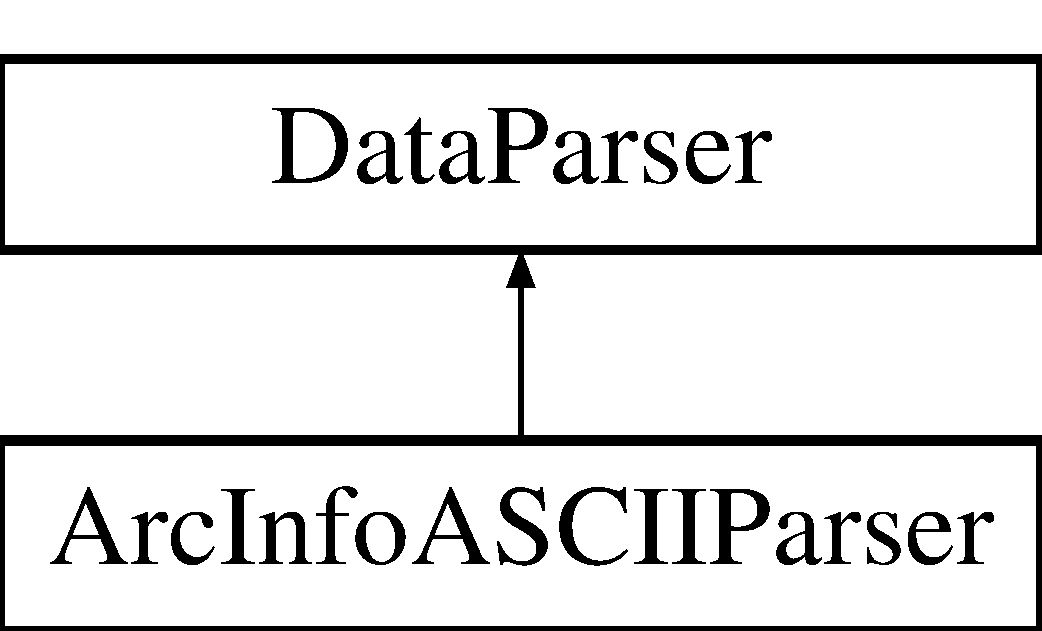
\includegraphics[height=2.000000cm]{classDataParser}
\end{center}
\end{figure}
\subsection*{\-Public \-Member \-Functions}
\begin{DoxyCompactItemize}
\item 
\hypertarget{classDataParser_adde3fdb08b6d298dac0bdf59b94d77c9}{\hyperlink{classDataParser_adde3fdb08b6d298dac0bdf59b94d77c9}{\-Data\-Parser} ()}\label{classDataParser_adde3fdb08b6d298dac0bdf59b94d77c9}

\begin{DoxyCompactList}\small\item\em default constructor \end{DoxyCompactList}\item 
\hypertarget{classDataParser_afbf1e7cdc1bde9fa75cdb4bead409c5f}{\hyperlink{classDataParser_afbf1e7cdc1bde9fa75cdb4bead409c5f}{\-Data\-Parser} (const string \&\-\_\-file\-Path)}\label{classDataParser_afbf1e7cdc1bde9fa75cdb4bead409c5f}

\begin{DoxyCompactList}\small\item\em overloaded constructor accept a parameter, setting the file path \end{DoxyCompactList}\item 
\hypertarget{classDataParser_a6df8b2ad220ec78e9a5155543392051a}{\hyperlink{classDataParser_a6df8b2ad220ec78e9a5155543392051a}{\-Data\-Parser} (const char $\ast$\-\_\-file\-Path)}\label{classDataParser_a6df8b2ad220ec78e9a5155543392051a}

\begin{DoxyCompactList}\small\item\em overloaded constructor accept one parameter, setting the file path \end{DoxyCompactList}\item 
\hypertarget{classDataParser_a4ac09e3a8b888b204e23052be8e1ec80}{virtual \hyperlink{classDataParser_a4ac09e3a8b888b204e23052be8e1ec80}{$\sim$\-Data\-Parser} ()}\label{classDataParser_a4ac09e3a8b888b204e23052be8e1ec80}

\begin{DoxyCompactList}\small\item\em destructor \end{DoxyCompactList}\item 
\hypertarget{classDataParser_a2d1d731f6e78f45a1d5e683aa2cc47c0}{void \hyperlink{classDataParser_a2d1d731f6e78f45a1d5e683aa2cc47c0}{set\-File\-Path} (const string \&\-\_\-file\-Path)}\label{classDataParser_a2d1d731f6e78f45a1d5e683aa2cc47c0}

\begin{DoxyCompactList}\small\item\em setter. set the file path \end{DoxyCompactList}\item 
\hypertarget{classDataParser_a0e65a165cd0144afe7c5fe68e71e090a}{void {\bfseries set\-File\-Path} (const char $\ast$\-\_\-file\-Path)}\label{classDataParser_a0e65a165cd0144afe7c5fe68e71e090a}

\item 
\hypertarget{classDataParser_aa16dd6e4395db13e1dc7a174a415ebc1}{string \hyperlink{classDataParser_aa16dd6e4395db13e1dc7a174a415ebc1}{get\-File\-Path} ()}\label{classDataParser_aa16dd6e4395db13e1dc7a174a415ebc1}

\begin{DoxyCompactList}\small\item\em getter. get the file path \end{DoxyCompactList}\item 
virtual bool \hyperlink{classDataParser_a45e498627eec0fc8638a34eab2ff2812}{parse} (\hyperlink{classGridLayer}{\-Grid\-Layer} \&gl, int multiplier=1)=0
\begin{DoxyCompactList}\small\item\em pure virtual member function used to parse data into a int-\/valued grirdlayer \end{DoxyCompactList}\end{DoxyCompactItemize}
\subsection*{\-Protected \-Attributes}
\begin{DoxyCompactItemize}
\item 
\hypertarget{classDataParser_a02f3f9f3cca1e56902b98dc2e39c7e22}{string {\bfseries file\-Path}}\label{classDataParser_a02f3f9f3cca1e56902b98dc2e39c7e22}

\end{DoxyCompactItemize}


\subsection{\-Detailed \-Description}
virtual class \hyperlink{classDataParser}{\-Data\-Parser} is used to parse various data file format, extracting corresponding data into grid layer 

currently, we only accept parse data from disk file, and the accepted file format should register in \-File\-Type structure, this is a function class, only provides some functions. 

\subsection{\-Member \-Function \-Documentation}
\hypertarget{classDataParser_a45e498627eec0fc8638a34eab2ff2812}{\index{\-Data\-Parser@{\-Data\-Parser}!parse@{parse}}
\index{parse@{parse}!DataParser@{\-Data\-Parser}}
\subsubsection[{parse}]{\setlength{\rightskip}{0pt plus 5cm}virtual bool {\bf \-Data\-Parser\-::parse} (
\begin{DoxyParamCaption}
\item[{{\bf \-Grid\-Layer} \&}]{gl, }
\item[{int}]{multiplier = {\ttfamily 1}}
\end{DoxyParamCaption}
)\hspace{0.3cm}{\ttfamily  \mbox{[}pure virtual\mbox{]}}}}\label{classDataParser_a45e498627eec0fc8638a34eab2ff2812}


pure virtual member function used to parse data into a int-\/valued grirdlayer 


\begin{DoxyParams}{\-Parameters}
{\em file\-Path} & the file path in disk \\
\hline
{\em gl} & the integer-\/valued grid layer to extract data to \\
\hline
{\em multiplier} & sometime all data in data file are small double, say 0.\-0032, the user can designate a multiplier, say 10000, then all data in grid layer will be multiplied by this multiplier, default to 1 \\
\hline
\end{DoxyParams}
\begin{DoxyReturn}{\-Returns}
true means successful, otherwise failed 
\end{DoxyReturn}


\-Implemented in \hyperlink{classArcInfoASCIIParser_a1f63530762118826b85565479c98502a}{\-Arc\-Info\-A\-S\-C\-I\-I\-Parser}.



\-The documentation for this class was generated from the following files\-:\begin{DoxyCompactItemize}
\item 
include/\hyperlink{DataParser_8h}{\-Data\-Parser.\-h}\item 
src/\-Data\-Parser.\-cpp\end{DoxyCompactItemize}

\hypertarget{structArcInfoASCIIGenerator_1_1FileHeader}{\section{\-Arc\-Info\-A\-S\-C\-I\-I\-Generator\-:\-:\-File\-Header \-Struct \-Reference}
\label{structArcInfoASCIIGenerator_1_1FileHeader}\index{\-Arc\-Info\-A\-S\-C\-I\-I\-Generator\-::\-File\-Header@{\-Arc\-Info\-A\-S\-C\-I\-I\-Generator\-::\-File\-Header}}
}


file header for \-Arc/\-Info \-A\-S\-C\-I\-I file format  




{\ttfamily \#include $<$\-Arc\-Info\-A\-S\-C\-I\-I\-Generator.\-h$>$}

\subsection*{\-Public \-Member \-Functions}
\begin{DoxyCompactItemize}
\item 
\hypertarget{structArcInfoASCIIGenerator_1_1FileHeader_aee1a0a9583333dc3f6e10d3a297386ff}{{\bfseries \-File\-Header} (int \-\_\-n\-Cols, int \-\_\-n\-Rows, double \-\_\-xll\-Corner, double \-\_\-yll\-Corner, double \-\_\-cell\-Size, int \-\_\-no\-Value)}\label{structArcInfoASCIIGenerator_1_1FileHeader_aee1a0a9583333dc3f6e10d3a297386ff}

\end{DoxyCompactItemize}
\subsection*{\-Public \-Attributes}
\begin{DoxyCompactItemize}
\item 
\hypertarget{structArcInfoASCIIGenerator_1_1FileHeader_a92571f6afaab2da4ffb03f8841aa1467}{int {\bfseries n\-Cols}}\label{structArcInfoASCIIGenerator_1_1FileHeader_a92571f6afaab2da4ffb03f8841aa1467}

\item 
\hypertarget{structArcInfoASCIIGenerator_1_1FileHeader_a00460ad3a53c48556aa7a7078faa42fa}{int \hyperlink{structArcInfoASCIIGenerator_1_1FileHeader_a00460ad3a53c48556aa7a7078faa42fa}{n\-Rows}}\label{structArcInfoASCIIGenerator_1_1FileHeader_a00460ad3a53c48556aa7a7078faa42fa}

\begin{DoxyCompactList}\small\item\em denote the number of rows and columns in data file \end{DoxyCompactList}\item 
\hypertarget{structArcInfoASCIIGenerator_1_1FileHeader_a61c3e83931884a290ab7e8b5370ff98f}{double {\bfseries xll\-Corner}}\label{structArcInfoASCIIGenerator_1_1FileHeader_a61c3e83931884a290ab7e8b5370ff98f}

\item 
\hypertarget{structArcInfoASCIIGenerator_1_1FileHeader_a6a477f07548715d424bc7d6dc04b4c7e}{double \hyperlink{structArcInfoASCIIGenerator_1_1FileHeader_a6a477f07548715d424bc7d6dc04b4c7e}{yll\-Corner}}\label{structArcInfoASCIIGenerator_1_1FileHeader_a6a477f07548715d424bc7d6dc04b4c7e}

\begin{DoxyCompactList}\small\item\em the x, y value for the left-\/bottom point( or center point) of the left bottom cell \end{DoxyCompactList}\item 
\hypertarget{structArcInfoASCIIGenerator_1_1FileHeader_a765a78b8364c349bf7f956a8082d93ca}{double \hyperlink{structArcInfoASCIIGenerator_1_1FileHeader_a765a78b8364c349bf7f956a8082d93ca}{cell\-Size}}\label{structArcInfoASCIIGenerator_1_1FileHeader_a765a78b8364c349bf7f956a8082d93ca}

\begin{DoxyCompactList}\small\item\em the cell size of the cell \end{DoxyCompactList}\item 
\hypertarget{structArcInfoASCIIGenerator_1_1FileHeader_a0e2ab90e13dd7ab96688c08da388a307}{int \hyperlink{structArcInfoASCIIGenerator_1_1FileHeader_a0e2ab90e13dd7ab96688c08da388a307}{no\-Value}}\label{structArcInfoASCIIGenerator_1_1FileHeader_a0e2ab90e13dd7ab96688c08da388a307}

\begin{DoxyCompactList}\small\item\em the same as \-Arc/\-Info \-A\-S\-C\-I\-I file \end{DoxyCompactList}\end{DoxyCompactItemize}
\subsection*{\-Friends}
\begin{DoxyCompactItemize}
\item 
\hypertarget{structArcInfoASCIIGenerator_1_1FileHeader_ad915f5c60819769ec761078664f42227}{ostream \& {\bfseries operator$<$$<$} (ostream \&os, const \hyperlink{structArcInfoASCIIGenerator_1_1FileHeader}{\-File\-Header} \&fh)}\label{structArcInfoASCIIGenerator_1_1FileHeader_ad915f5c60819769ec761078664f42227}

\item 
\hypertarget{structArcInfoASCIIGenerator_1_1FileHeader_a4f321889db256758ae5ef68527a1e698}{istream \& {\bfseries operator$>$$>$} (istream \&is, \hyperlink{structArcInfoASCIIGenerator_1_1FileHeader}{\-File\-Header} \&fh)}\label{structArcInfoASCIIGenerator_1_1FileHeader_a4f321889db256758ae5ef68527a1e698}

\end{DoxyCompactItemize}


\subsection{\-Detailed \-Description}
file header for \-Arc/\-Info \-A\-S\-C\-I\-I file format 

\-This structure contains self describle members which correpsond to real \-Arc/\-Info \-A\-S\-C\-I\-I file header 

\-The documentation for this struct was generated from the following file\-:\begin{DoxyCompactItemize}
\item 
include/\hyperlink{ArcInfoASCIIGenerator_8h}{\-Arc\-Info\-A\-S\-C\-I\-I\-Generator.\-h}\end{DoxyCompactItemize}

\hypertarget{classGenerateBlock}{\section{\-Generate\-Block \-Class \-Reference}
\label{classGenerateBlock}\index{\-Generate\-Block@{\-Generate\-Block}}
}


class \hyperlink{classGenerateBlock}{\-Generate\-Block} is used to generate \-Blocks from interpolated \hyperlink{classGridLayer}{\-Grid\-Layer}  




{\ttfamily \#include $<$\-Generate\-Block.\-h$>$}

\subsection*{\-Public \-Member \-Functions}
\begin{DoxyCompactItemize}
\item 
bool \hyperlink{classGenerateBlock_a03b4af01be301dc88176c125a91c3a83}{generate} (\hyperlink{classGridLayer}{\-Grid\-Layer} \&gl, \hyperlink{classInterpolate}{\-Interpolate} \&tool, vector$<$ \hyperlink{classBlock}{\-Block} $>$ \&result, int value, int interval\-Index)
\begin{DoxyCompactList}\small\item\em this function use specified interpolating algorithm to interpolate \hyperlink{classGridLayer}{\-Grid\-Layer}, then extract all \-Blocks. \-Blocks which have the same interior value will be stored in the same 1\-D array. \end{DoxyCompactList}\end{DoxyCompactItemize}


\subsection{\-Detailed \-Description}
class \hyperlink{classGenerateBlock}{\-Generate\-Block} is used to generate \-Blocks from interpolated \hyperlink{classGridLayer}{\-Grid\-Layer} 

\-This class only provide methods, so it's a functional class 

\subsection{\-Member \-Function \-Documentation}
\hypertarget{classGenerateBlock_a03b4af01be301dc88176c125a91c3a83}{\index{\-Generate\-Block@{\-Generate\-Block}!generate@{generate}}
\index{generate@{generate}!GenerateBlock@{\-Generate\-Block}}
\subsubsection[{generate}]{\setlength{\rightskip}{0pt plus 5cm}bool {\bf \-Generate\-Block\-::generate} (
\begin{DoxyParamCaption}
\item[{{\bf \-Grid\-Layer} \&}]{gl, }
\item[{{\bf \-Interpolate} \&}]{tool, }
\item[{vector$<$ {\bf \-Block} $>$ \&}]{result, }
\item[{int}]{value, }
\item[{int}]{interval\-Index}
\end{DoxyParamCaption}
)}}\label{classGenerateBlock_a03b4af01be301dc88176c125a91c3a83}


this function use specified interpolating algorithm to interpolate \hyperlink{classGridLayer}{\-Grid\-Layer}, then extract all \-Blocks. \-Blocks which have the same interior value will be stored in the same 1\-D array. 


\begin{DoxyParams}{\-Parameters}
{\em gl.} & gl is \hyperlink{classGridLayer}{\-Grid\-Layer} instantiation \\
\hline
{\em tool.} & tool is interpolating algorithm \\
\hline
{\em result.} & result is a 1\-D array, will store \-Blocks have the same interior value equal to \char`\"{}value\char`\"{} \\
\hline
{\em value.} & specified the value you are interested \\
\hline
{\em interval\-Index.} & specific the interval layer you are interested \\
\hline
\end{DoxyParams}
\begin{DoxyReturn}{\-Returns}
true means successfully generate all blocks, false means failed 
\end{DoxyReturn}


\-The documentation for this class was generated from the following files\-:\begin{DoxyCompactItemize}
\item 
include/\hyperlink{GenerateBlock_8h}{\-Generate\-Block.\-h}\item 
src/\-Generate\-Block.\-cpp\end{DoxyCompactItemize}

\hypertarget{classGenerateVolume}{\section{\-Generate\-Volume \-Class \-Reference}
\label{classGenerateVolume}\index{\-Generate\-Volume@{\-Generate\-Volume}}
}


this class is used to generate volumes  




{\ttfamily \#include $<$\-Generate\-Volume.\-h$>$}

\subsection*{\-Public \-Member \-Functions}
\begin{DoxyCompactItemize}
\item 
bool \hyperlink{classGenerateVolume_a1c4a1b9928188dd96f33f611d41ef22a}{generate} (\hyperlink{classGridLayer}{\-Grid\-Layer} \&gl, \hyperlink{classInterpolate}{\-Interpolate} \&tool, vector$<$ \hyperlink{classVolume}{\-Volume} $>$ \&result, int value, int interval\-Index)
\begin{DoxyCompactList}\small\item\em this function is used to generate volumes which have the specified value. \-All extracting volumes will be stored in 1\-D array and these volumes must exist in specified interval \end{DoxyCompactList}\end{DoxyCompactItemize}


\subsection{\-Detailed \-Description}
this class is used to generate volumes 

\-This class only provide methods, so only member function delcarations exist 

\subsection{\-Member \-Function \-Documentation}
\hypertarget{classGenerateVolume_a1c4a1b9928188dd96f33f611d41ef22a}{\index{\-Generate\-Volume@{\-Generate\-Volume}!generate@{generate}}
\index{generate@{generate}!GenerateVolume@{\-Generate\-Volume}}
\subsubsection[{generate}]{\setlength{\rightskip}{0pt plus 5cm}bool {\bf \-Generate\-Volume\-::generate} (
\begin{DoxyParamCaption}
\item[{{\bf \-Grid\-Layer} \&}]{gl, }
\item[{{\bf \-Interpolate} \&}]{tool, }
\item[{vector$<$ {\bf \-Volume} $>$ \&}]{result, }
\item[{int}]{value, }
\item[{int}]{interval\-Index}
\end{DoxyParamCaption}
)}}\label{classGenerateVolume_a1c4a1b9928188dd96f33f611d41ef22a}


this function is used to generate volumes which have the specified value. \-All extracting volumes will be stored in 1\-D array and these volumes must exist in specified interval 


\begin{DoxyParams}{\-Parameters}
{\em gl.} & gl provide the \hyperlink{classGridLayer}{\-Grid\-Layer} we are working on \\
\hline
{\em tool.} & tool is the interpolating algorithm we are using to interpolate the gl \\
\hline
{\em result.} & result is 1\-D array, stores all extracting volumes \\
\hline
{\em value.} & value specify the interior value we are interested in \\
\hline
{\em interval\-Index.} & interval\-Index specify the interval of the gl we are interested in, must range from \char`\"{}0\char`\"{}(included) to \char`\"{}gl.\-get\-Num\-Of\-Layers()-\/2\char`\"{}(included \\
\hline
\end{DoxyParams}
\begin{DoxyReturn}{\-Returns}
true means extracting specified volumes successfully, otherwise falied 
\end{DoxyReturn}


\-The documentation for this class was generated from the following files\-:\begin{DoxyCompactItemize}
\item 
include/\hyperlink{GenerateVolume_8h}{\-Generate\-Volume.\-h}\item 
src/\-Generate\-Volume.\-cpp\end{DoxyCompactItemize}

\hypertarget{structGeometricInfo}{\section{\-Geometric\-Info \-Struct \-Reference}
\label{structGeometricInfo}\index{\-Geometric\-Info@{\-Geometric\-Info}}
}


\hyperlink{structGeometricInfo}{\-Geometric\-Info} data structure is used to record ths geometric info about the grids in a grid layer.  




{\ttfamily \#include $<$\-Grid\-Layer.\-h$>$}

\subsection*{\-Public \-Member \-Functions}
\begin{DoxyCompactItemize}
\item 
\hypertarget{structGeometricInfo_a4bc847dd106d32107fde0c0d2fa00f77}{\hyperlink{structGeometricInfo_a4bc847dd106d32107fde0c0d2fa00f77}{\-Geometric\-Info} ()}\label{structGeometricInfo_a4bc847dd106d32107fde0c0d2fa00f77}

\begin{DoxyCompactList}\small\item\em default constructor \end{DoxyCompactList}\item 
\hypertarget{structGeometricInfo_aaa47b9cbf705ec7a20f6895721b8158f}{\hyperlink{structGeometricInfo_aaa47b9cbf705ec7a20f6895721b8158f}{\-Geometric\-Info} (double \-\_\-longitude, double \-\_\-latitude, double \-\_\-cell\-Size, \-Metric \-\_\-cell\-Metric)}\label{structGeometricInfo_aaa47b9cbf705ec7a20f6895721b8158f}

\begin{DoxyCompactList}\small\item\em overloaded constructor \end{DoxyCompactList}\item 
\hypertarget{structGeometricInfo_a996d4f1cb6b640cce436a982d400d0ad}{\hyperlink{structGeometricInfo_a996d4f1cb6b640cce436a982d400d0ad}{\-Geometric\-Info} (double \-\_\-longitude, double \-\_\-latitude, double \-\_\-cell\-Length, double \-\_\-cell\-Width)}\label{structGeometricInfo_a996d4f1cb6b640cce436a982d400d0ad}

\begin{DoxyCompactList}\small\item\em overloaded constructor \end{DoxyCompactList}\item 
\hypertarget{structGeometricInfo_a210973010d9c0e049e5ee7308b748358}{\hyperlink{structGeometricInfo_a210973010d9c0e049e5ee7308b748358}{\-Geometric\-Info} (double \-\_\-longitude, double \-\_\-latitude, double \-\_\-cell\-Length, \-Metric \-\_\-cell\-Length\-Metric, double \-\_\-cell\-Width, \-Metric \-\_\-cell\-Width\-Metric)}\label{structGeometricInfo_a210973010d9c0e049e5ee7308b748358}

\begin{DoxyCompactList}\small\item\em overloaded constructor \end{DoxyCompactList}\item 
\hypertarget{structGeometricInfo_a004bf2571153dca81c1a36950f1cb9e7}{\hyperlink{structGeometricInfo}{\-Geometric\-Info} \& \hyperlink{structGeometricInfo_a004bf2571153dca81c1a36950f1cb9e7}{operator=} (const \hyperlink{structGeometricInfo}{\-Geometric\-Info} \&right)}\label{structGeometricInfo_a004bf2571153dca81c1a36950f1cb9e7}

\begin{DoxyCompactList}\small\item\em assignment operator \end{DoxyCompactList}\end{DoxyCompactItemize}
\subsection*{\-Public \-Attributes}
\begin{DoxyCompactItemize}
\item 
\hypertarget{structGeometricInfo_a91a5b4f492552e00f00e95293dd173f3}{double \hyperlink{structGeometricInfo_a91a5b4f492552e00f00e95293dd173f3}{longitude}}\label{structGeometricInfo_a91a5b4f492552e00f00e95293dd173f3}

\begin{DoxyCompactList}\small\item\em longitude of the origin \end{DoxyCompactList}\item 
\hypertarget{structGeometricInfo_afea47fa5d5a23432ba84b5fba8ddea7f}{double \hyperlink{structGeometricInfo_afea47fa5d5a23432ba84b5fba8ddea7f}{latitude}}\label{structGeometricInfo_afea47fa5d5a23432ba84b5fba8ddea7f}

\begin{DoxyCompactList}\small\item\em latitude of the origin \end{DoxyCompactList}\item 
\hypertarget{structGeometricInfo_a7d1c03e44c33b4b65eaf5541b3ce60ba}{double \hyperlink{structGeometricInfo_a7d1c03e44c33b4b65eaf5541b3ce60ba}{cell\-Length}}\label{structGeometricInfo_a7d1c03e44c33b4b65eaf5541b3ce60ba}

\begin{DoxyCompactList}\small\item\em length of the cell \end{DoxyCompactList}\item 
\hypertarget{structGeometricInfo_aee3e7c10cb0746a3d61097d3454895c2}{\-Metric \hyperlink{structGeometricInfo_aee3e7c10cb0746a3d61097d3454895c2}{cell\-Length\-Metric}}\label{structGeometricInfo_aee3e7c10cb0746a3d61097d3454895c2}

\begin{DoxyCompactList}\small\item\em metric used by cell length \end{DoxyCompactList}\item 
\hypertarget{structGeometricInfo_abc44fb6574fa395a5df1d655a689c237}{double \hyperlink{structGeometricInfo_abc44fb6574fa395a5df1d655a689c237}{cell\-Width}}\label{structGeometricInfo_abc44fb6574fa395a5df1d655a689c237}

\begin{DoxyCompactList}\small\item\em width of the cell \end{DoxyCompactList}\item 
\hypertarget{structGeometricInfo_aeaacb3aef4f2406491a732761fc2fbb3}{\-Metric \hyperlink{structGeometricInfo_aeaacb3aef4f2406491a732761fc2fbb3}{cell\-Width\-Metric}}\label{structGeometricInfo_aeaacb3aef4f2406491a732761fc2fbb3}

\begin{DoxyCompactList}\small\item\em metric used by cell \char`\"{}width\char`\"{} \end{DoxyCompactList}\end{DoxyCompactItemize}


\subsection{\-Detailed \-Description}
\hyperlink{structGeometricInfo}{\-Geometric\-Info} data structure is used to record ths geometric info about the grids in a grid layer. 

\-The grids in a gridlayer have some geometric info, such as the origin, the metric, the cell size. \-All grids in a gridlayer should be homogeneous, this means the grids should not only have the same rows and columns, but also have the some origin, cell size, metric. 

\-The documentation for this struct was generated from the following file\-:\begin{DoxyCompactItemize}
\item 
include/\hyperlink{GridLayer_8h}{\-Grid\-Layer.\-h}\end{DoxyCompactItemize}

\hypertarget{classGridLayer}{\section{\-Grid\-Layer \-Class \-Reference}
\label{classGridLayer}\index{\-Grid\-Layer@{\-Grid\-Layer}}
}


class accept only integer value.  




{\ttfamily \#include $<$\-Grid\-Layer.\-h$>$}

\subsection*{\-Public \-Member \-Functions}
\begin{DoxyCompactItemize}
\item 
\hypertarget{classGridLayer_ad58adca9bc030db555ed8e71b41a0332}{\hyperlink{classGridLayer_ad58adca9bc030db555ed8e71b41a0332}{\-Grid\-Layer} ()}\label{classGridLayer_ad58adca9bc030db555ed8e71b41a0332}

\begin{DoxyCompactList}\small\item\em default constructor \end{DoxyCompactList}\item 
\hyperlink{classGridLayer_a7a731b2b9efbae6deab063dd5af83293}{\-Grid\-Layer} (int layer, int row, int col, double height\-Interval, long long value)
\begin{DoxyCompactList}\small\item\em constructor to set detailed info for the grid layer \end{DoxyCompactList}\item 
\hypertarget{classGridLayer_ab4662377f5de2bfe0a554f057187b08d}{\hyperlink{classGridLayer_ab4662377f5de2bfe0a554f057187b08d}{\-Grid\-Layer} (const vector$<$ vector$<$ vector$<$ long long $>$ $>$ $>$ \&argu, double height\-Interval)}\label{classGridLayer_ab4662377f5de2bfe0a554f057187b08d}

\begin{DoxyCompactList}\small\item\em copy constructor \end{DoxyCompactList}\item 
\hypertarget{classGridLayer_a26ef976a6b5e2bc2959404284495619b}{\hyperlink{classGridLayer_a26ef976a6b5e2bc2959404284495619b}{$\sim$\-Grid\-Layer} ()}\label{classGridLayer_a26ef976a6b5e2bc2959404284495619b}

\begin{DoxyCompactList}\small\item\em destructor \end{DoxyCompactList}\item 
int \hyperlink{classGridLayer_a692d934e688b38feafbd8e80d301a596}{get\-Num\-Of\-Layers} ()
\begin{DoxyCompactList}\small\item\em $>$ getter. return number of layers \end{DoxyCompactList}\item 
int \hyperlink{classGridLayer_adbb8ed986a96063e3c986fb474db2ad7}{get\-Num\-Of\-Rows} ()
\begin{DoxyCompactList}\small\item\em $>$ getter. return number of rows for each layer. each layer should have the same number of rows \end{DoxyCompactList}\item 
int \hyperlink{classGridLayer_aafa4cad0c7572dd5df051daaa6480b52}{get\-Num\-Of\-Columns} ()
\begin{DoxyCompactList}\small\item\em $>$ getter. return number of columns for each layer. each layer should have the same number of columns \end{DoxyCompactList}\item 
double \hyperlink{classGridLayer_ab18678e9be40fe08e34002b24e4541a8}{get\-Height\-Interval} ()
\begin{DoxyCompactList}\small\item\em $>$ getter. return the height between adjacent layers, \char`\"{}n\char`\"{} layers have \char`\"{}n-\/1\char`\"{} intervals \end{DoxyCompactList}\item 
\hypertarget{classGridLayer_a5c00efe20cc10be6479381f1855e459b}{\-Metric \hyperlink{classGridLayer_a5c00efe20cc10be6479381f1855e459b}{get\-Height\-Interval\-Metric} ()}\label{classGridLayer_a5c00efe20cc10be6479381f1855e459b}

\begin{DoxyCompactList}\small\item\em $>$ getter. return the metric used by \char`\"{}height\-Interval\char`\"{}, could be \char`\"{}\-M\-E\-T\-E\-R\char`\"{}, \char`\"{}\-K\-I\-L\-O\-M\-E\-T\-E\-R\char`\"{} or \char`\"{}\-M\-I\-L\-E\char`\"{} \end{DoxyCompactList}\item 
\hypertarget{classGridLayer_a7b190d6edef6697c3fe1b2bf6cbee639}{double \hyperlink{classGridLayer_a7b190d6edef6697c3fe1b2bf6cbee639}{get\-Ground\-To\-Lowest\-Layer} ()}\label{classGridLayer_a7b190d6edef6697c3fe1b2bf6cbee639}

\begin{DoxyCompactList}\small\item\em $>$ getter. return the height between earth surface to the lowest layer \end{DoxyCompactList}\item 
\hypertarget{classGridLayer_a51585377aaa1a7a72f6b2e516f22cdfb}{\-Metric \hyperlink{classGridLayer_a51585377aaa1a7a72f6b2e516f22cdfb}{get\-Ground\-To\-Lowest\-Layer\-Metric} ()}\label{classGridLayer_a51585377aaa1a7a72f6b2e516f22cdfb}

\begin{DoxyCompactList}\small\item\em $>$ getter. return the metric used by \char`\"{}ground\-To\-Lowest\-Layer\char`\"{}, could be \char`\"{}\-M\-E\-T\-E\-R\char`\"{}, \char`\"{}\-K\-I\-L\-O\-E\-M\-E\-T\-E\-R\char`\"{} or \char`\"{}\-M\-I\-L\-E\char`\"{} \end{DoxyCompactList}\item 
\hypertarget{classGridLayer_aa66a23f509e0fbe737b61477eb183110}{vector$<$ vector$<$ vector$<$ long \*
long $>$ $>$ $>$ \hyperlink{classGridLayer_aa66a23f509e0fbe737b61477eb183110}{get\-All\-Layers} ()}\label{classGridLayer_aa66a23f509e0fbe737b61477eb183110}

\begin{DoxyCompactList}\small\item\em $>$ getter. return all layers as 3\-D matrix \end{DoxyCompactList}\item 
vector$<$ vector$<$ long long $>$ $>$ \hyperlink{classGridLayer_a4d8fc5058d310668b52decd3dabfd95e}{get\-Specific\-Layer} (int layer)
\begin{DoxyCompactList}\small\item\em $>$ getter. return a specific layer as 2\-D matrix \end{DoxyCompactList}\item 
long long \hyperlink{classGridLayer_a9f83a516dacd8030957dd1d70474bc60}{get\-Cell\-Value} (int layer, int row, int col)
\begin{DoxyCompactList}\small\item\em $>$ getter. return value stored in a specific cell \end{DoxyCompactList}\item 
\hypertarget{classGridLayer_a36ceb6db89b190d4575f6f54809c39b8}{\hyperlink{structDataInfo}{\-Data\-Info} \hyperlink{classGridLayer_a36ceb6db89b190d4575f6f54809c39b8}{get\-Data\-Info} ()}\label{classGridLayer_a36ceb6db89b190d4575f6f54809c39b8}

\begin{DoxyCompactList}\small\item\em $>$ getter. get the data info \end{DoxyCompactList}\item 
\hypertarget{classGridLayer_a3d576c2329066b7aaabfaaffdb2b1f54}{\hyperlink{structGeometricInfo}{\-Geometric\-Info} \hyperlink{classGridLayer_a3d576c2329066b7aaabfaaffdb2b1f54}{get\-Geometric\-Info} ()}\label{classGridLayer_a3d576c2329066b7aaabfaaffdb2b1f54}

\begin{DoxyCompactList}\small\item\em $>$ getter. get the geometric info \end{DoxyCompactList}\item 
void \hyperlink{classGridLayer_a7c76d709457ea5bf6d87f1d9f4bfa95a}{set\-All\-Layers} (const vector$<$ vector$<$ vector$<$ long long $>$ $>$ $>$ \&argu)
\begin{DoxyCompactList}\small\item\em $>$ setter. set all layers \end{DoxyCompactList}\item 
void \hyperlink{classGridLayer_a7f5c9e2435213374d1a406b825f18726}{set\-Specific\-Layer} (int index, const vector$<$ vector$<$ long long $>$ $>$ \&argu)
\begin{DoxyCompactList}\small\item\em $>$ setter. set specific layer. \char`\"{}index\char`\"{} must only vary from \char`\"{}0\char`\"{} to \char`\"{}get\-Num\-Of\-Layers()\char`\"{}(included) \end{DoxyCompactList}\item 
void \hyperlink{classGridLayer_a8d94cee990ba0d799d17f26501bdc473}{set\-Height\-Interval} (double height)
\begin{DoxyCompactList}\small\item\em $>$ setter. set the height interval between every adjacent layers \end{DoxyCompactList}\item 
\hypertarget{classGridLayer_a2e9aca476dadc47333e26e2f036e1932}{void \hyperlink{classGridLayer_a2e9aca476dadc47333e26e2f036e1932}{set\-Height\-Interval\-Metric} (\-Metric metric)}\label{classGridLayer_a2e9aca476dadc47333e26e2f036e1932}

\begin{DoxyCompactList}\small\item\em $>$ setter. set the metric used by \char`\"{}height\-Interval\char`\"{} \end{DoxyCompactList}\item 
\hypertarget{classGridLayer_a63520a28c62328e6bc30c0d98d8f54da}{void \hyperlink{classGridLayer_a63520a28c62328e6bc30c0d98d8f54da}{set\-Ground\-To\-Lowest\-Layer} (double \-\_\-ground\-To\-Lowest\-Layer)}\label{classGridLayer_a63520a28c62328e6bc30c0d98d8f54da}

\begin{DoxyCompactList}\small\item\em $>$ setter. set the height between earth surface to the lowest layer \end{DoxyCompactList}\item 
\hypertarget{classGridLayer_abce744494d0c6588242ae7bd9a1231fa}{void \hyperlink{classGridLayer_abce744494d0c6588242ae7bd9a1231fa}{set\-Ground\-To\-Lowest\-Layer\-Metric} (\-Metric metric)}\label{classGridLayer_abce744494d0c6588242ae7bd9a1231fa}

\begin{DoxyCompactList}\small\item\em $>$ setter. set the metric used by \char`\"{}ground\-To\-Lowest\-Layer\char`\"{} \end{DoxyCompactList}\item 
void \hyperlink{classGridLayer_a7dbf9877fce98d4dd9d29575643c2c2c}{set\-Cell\-Value} (int layer, int row, int col, long long new\-Value)
\begin{DoxyCompactList}\small\item\em $>$ setter. set new value for a specific cell \end{DoxyCompactList}\item 
\hypertarget{classGridLayer_a63145fba564be57678273e9bae1cacac}{void \hyperlink{classGridLayer_a63145fba564be57678273e9bae1cacac}{set\-Data\-Info} (const \hyperlink{structDataInfo}{\-Data\-Info} \&argu)}\label{classGridLayer_a63145fba564be57678273e9bae1cacac}

\begin{DoxyCompactList}\small\item\em $>$ setter. set the data\-Info \end{DoxyCompactList}\item 
\hypertarget{classGridLayer_a6e324a08ae12b96c8591149a28d82ff4}{void \hyperlink{classGridLayer_a6e324a08ae12b96c8591149a28d82ff4}{set\-Geometric\-Info} (const \hyperlink{structGeometricInfo}{\-Geometric\-Info} \&argu)}\label{classGridLayer_a6e324a08ae12b96c8591149a28d82ff4}

\begin{DoxyCompactList}\small\item\em $>$ setter. set the geometric\-Info \end{DoxyCompactList}\item 
\hypertarget{classGridLayer_a5d8428e905e0d016b4dd02b5ced48ecb}{bool \hyperlink{classGridLayer_a5d8428e905e0d016b4dd02b5ced48ecb}{insert\-Layer} (const vector$<$ vector$<$ long long $>$ $>$ \&tmp, int layer\-Index)}\label{classGridLayer_a5d8428e905e0d016b4dd02b5ced48ecb}

\begin{DoxyCompactList}\small\item\em $>$ insert new layer into a index, \char`\"{}layer\-Index\char`\"{} should range from 0 to \hyperlink{classGridLayer_a692d934e688b38feafbd8e80d301a596}{get\-Num\-Of\-Layers()} (included) \end{DoxyCompactList}\item 
\hypertarget{classGridLayer_a71d212f3683740c1789177817272223a}{bool \hyperlink{classGridLayer_a71d212f3683740c1789177817272223a}{delete\-Layer} (int layer\-Index)}\label{classGridLayer_a71d212f3683740c1789177817272223a}

\begin{DoxyCompactList}\small\item\em $>$ delete a layer, \char`\"{}layer\-Index\char`\"{} should range from 0 to \char`\"{}get\-Num\-Of\-Layers()-\/1\char`\"{} (included) \end{DoxyCompactList}\end{DoxyCompactItemize}


\subsection{\-Detailed \-Description}
class accept only integer value. 

\-Currently, the grid layer only store \char`\"{}long long int\char`\"{} type. \-Later we may resort to external library \char`\"{}big\-Int\char`\"{} in case of large integers 

\subsection{\-Constructor \& \-Destructor \-Documentation}
\hypertarget{classGridLayer_a7a731b2b9efbae6deab063dd5af83293}{\index{\-Grid\-Layer@{\-Grid\-Layer}!\-Grid\-Layer@{\-Grid\-Layer}}
\index{\-Grid\-Layer@{\-Grid\-Layer}!GridLayer@{\-Grid\-Layer}}
\subsubsection[{\-Grid\-Layer}]{\setlength{\rightskip}{0pt plus 5cm}{\bf \-Grid\-Layer\-::\-Grid\-Layer} (
\begin{DoxyParamCaption}
\item[{int}]{layer, }
\item[{int}]{row, }
\item[{int}]{col, }
\item[{double}]{\-\_\-height\-Interval, }
\item[{long long}]{value}
\end{DoxyParamCaption}
)}}\label{classGridLayer_a7a731b2b9efbae6deab063dd5af83293}


constructor to set detailed info for the grid layer 


\begin{DoxyParams}{\-Parameters}
{\em layer} & the number of layers in the grid layer \\
\hline
{\em row} & the number of rows in one layer \\
\hline
{\em col} & the number of columns in one layer \\
\hline
{\em value} & the value in all cells \\
\hline
\end{DoxyParams}


\subsection{\-Member \-Function \-Documentation}
\hypertarget{classGridLayer_a9f83a516dacd8030957dd1d70474bc60}{\index{\-Grid\-Layer@{\-Grid\-Layer}!get\-Cell\-Value@{get\-Cell\-Value}}
\index{get\-Cell\-Value@{get\-Cell\-Value}!GridLayer@{\-Grid\-Layer}}
\subsubsection[{get\-Cell\-Value}]{\setlength{\rightskip}{0pt plus 5cm}long long {\bf \-Grid\-Layer\-::get\-Cell\-Value} (
\begin{DoxyParamCaption}
\item[{int}]{layer, }
\item[{int}]{row, }
\item[{int}]{col}
\end{DoxyParamCaption}
)}}\label{classGridLayer_a9f83a516dacd8030957dd1d70474bc60}


$>$ getter. return value stored in a specific cell 

get specific cell value in the grid layer


\begin{DoxyParams}{\-Parameters}
{\em layer} & index of the layer, remember the index starts from 0, if out of bound, error! \\
\hline
{\em row} & row of the wanted cell \\
\hline
{\em col} & column of the wanted cell \\
\hline
\end{DoxyParams}
\begin{DoxyReturn}{\-Returns}
value stored in specific cell 
\end{DoxyReturn}
\hypertarget{classGridLayer_ab18678e9be40fe08e34002b24e4541a8}{\index{\-Grid\-Layer@{\-Grid\-Layer}!get\-Height\-Interval@{get\-Height\-Interval}}
\index{get\-Height\-Interval@{get\-Height\-Interval}!GridLayer@{\-Grid\-Layer}}
\subsubsection[{get\-Height\-Interval}]{\setlength{\rightskip}{0pt plus 5cm}double {\bf \-Grid\-Layer\-::get\-Height\-Interval} (
\begin{DoxyParamCaption}
{}
\end{DoxyParamCaption}
)}}\label{classGridLayer_ab18678e9be40fe08e34002b24e4541a8}


$>$ getter. return the height between adjacent layers, \char`\"{}n\char`\"{} layers have \char`\"{}n-\/1\char`\"{} intervals 

getter. get the height interval between two adjacent grids \hypertarget{classGridLayer_aafa4cad0c7572dd5df051daaa6480b52}{\index{\-Grid\-Layer@{\-Grid\-Layer}!get\-Num\-Of\-Columns@{get\-Num\-Of\-Columns}}
\index{get\-Num\-Of\-Columns@{get\-Num\-Of\-Columns}!GridLayer@{\-Grid\-Layer}}
\subsubsection[{get\-Num\-Of\-Columns}]{\setlength{\rightskip}{0pt plus 5cm}int {\bf \-Grid\-Layer\-::get\-Num\-Of\-Columns} (
\begin{DoxyParamCaption}
{}
\end{DoxyParamCaption}
)}}\label{classGridLayer_aafa4cad0c7572dd5df051daaa6480b52}


$>$ getter. return number of columns for each layer. each layer should have the same number of columns 

getter, get number of columns in one layer.

\begin{DoxyReturn}{\-Returns}
-\/1 means grid layer holds nothing, otherwise greater than 0 
\end{DoxyReturn}
\hypertarget{classGridLayer_a692d934e688b38feafbd8e80d301a596}{\index{\-Grid\-Layer@{\-Grid\-Layer}!get\-Num\-Of\-Layers@{get\-Num\-Of\-Layers}}
\index{get\-Num\-Of\-Layers@{get\-Num\-Of\-Layers}!GridLayer@{\-Grid\-Layer}}
\subsubsection[{get\-Num\-Of\-Layers}]{\setlength{\rightskip}{0pt plus 5cm}int {\bf \-Grid\-Layer\-::get\-Num\-Of\-Layers} (
\begin{DoxyParamCaption}
{}
\end{DoxyParamCaption}
)}}\label{classGridLayer_a692d934e688b38feafbd8e80d301a596}


$>$ getter. return number of layers 

getter. get number of layers in the grid layer \hypertarget{classGridLayer_adbb8ed986a96063e3c986fb474db2ad7}{\index{\-Grid\-Layer@{\-Grid\-Layer}!get\-Num\-Of\-Rows@{get\-Num\-Of\-Rows}}
\index{get\-Num\-Of\-Rows@{get\-Num\-Of\-Rows}!GridLayer@{\-Grid\-Layer}}
\subsubsection[{get\-Num\-Of\-Rows}]{\setlength{\rightskip}{0pt plus 5cm}int {\bf \-Grid\-Layer\-::get\-Num\-Of\-Rows} (
\begin{DoxyParamCaption}
{}
\end{DoxyParamCaption}
)}}\label{classGridLayer_adbb8ed986a96063e3c986fb474db2ad7}


$>$ getter. return number of rows for each layer. each layer should have the same number of rows 

getter, get number of rows in one layer.

\begin{DoxyReturn}{\-Returns}
-\/1 means grid layer holds nothing, otherwise greater than 0 
\end{DoxyReturn}
\hypertarget{classGridLayer_a4d8fc5058d310668b52decd3dabfd95e}{\index{\-Grid\-Layer@{\-Grid\-Layer}!get\-Specific\-Layer@{get\-Specific\-Layer}}
\index{get\-Specific\-Layer@{get\-Specific\-Layer}!GridLayer@{\-Grid\-Layer}}
\subsubsection[{get\-Specific\-Layer}]{\setlength{\rightskip}{0pt plus 5cm}vector$<$ vector$<$ long long $>$ $>$ {\bf \-Grid\-Layer\-::get\-Specific\-Layer} (
\begin{DoxyParamCaption}
\item[{int}]{layer}
\end{DoxyParamCaption}
)}}\label{classGridLayer_a4d8fc5058d310668b52decd3dabfd95e}


$>$ getter. return a specific layer as 2\-D matrix 

get specific layer in the gridlayer


\begin{DoxyParams}{\-Parameters}
{\em layer} & index starts from 0, so parameter should greater than -\/1 but must less than the number of layers, otherwise exit \\
\hline
\end{DoxyParams}
\begin{DoxyReturn}{\-Returns}
the wanted layer 
\end{DoxyReturn}
\hypertarget{classGridLayer_a7c76d709457ea5bf6d87f1d9f4bfa95a}{\index{\-Grid\-Layer@{\-Grid\-Layer}!set\-All\-Layers@{set\-All\-Layers}}
\index{set\-All\-Layers@{set\-All\-Layers}!GridLayer@{\-Grid\-Layer}}
\subsubsection[{set\-All\-Layers}]{\setlength{\rightskip}{0pt plus 5cm}void {\bf \-Grid\-Layer\-::set\-All\-Layers} (
\begin{DoxyParamCaption}
\item[{const vector$<$ vector$<$ vector$<$ long long $>$ $>$ $>$ \&}]{argu}
\end{DoxyParamCaption}
)}}\label{classGridLayer_a7c76d709457ea5bf6d87f1d9f4bfa95a}


$>$ setter. set all layers 

set grid layer \hypertarget{classGridLayer_a7dbf9877fce98d4dd9d29575643c2c2c}{\index{\-Grid\-Layer@{\-Grid\-Layer}!set\-Cell\-Value@{set\-Cell\-Value}}
\index{set\-Cell\-Value@{set\-Cell\-Value}!GridLayer@{\-Grid\-Layer}}
\subsubsection[{set\-Cell\-Value}]{\setlength{\rightskip}{0pt plus 5cm}void {\bf \-Grid\-Layer\-::set\-Cell\-Value} (
\begin{DoxyParamCaption}
\item[{int}]{layer, }
\item[{int}]{row, }
\item[{int}]{col, }
\item[{long long}]{new\-Value}
\end{DoxyParamCaption}
)}}\label{classGridLayer_a7dbf9877fce98d4dd9d29575643c2c2c}


$>$ setter. set new value for a specific cell 

set specific cell value


\begin{DoxyParams}{\-Parameters}
{\em layer} & the layer of the cell \\
\hline
{\em row} & the row of the cell \\
\hline
{\em col} & the column of the cell \\
\hline
{\em new\-Value} & the new value of the cell \\
\hline
\end{DoxyParams}
\hypertarget{classGridLayer_a8d94cee990ba0d799d17f26501bdc473}{\index{\-Grid\-Layer@{\-Grid\-Layer}!set\-Height\-Interval@{set\-Height\-Interval}}
\index{set\-Height\-Interval@{set\-Height\-Interval}!GridLayer@{\-Grid\-Layer}}
\subsubsection[{set\-Height\-Interval}]{\setlength{\rightskip}{0pt plus 5cm}void {\bf \-Grid\-Layer\-::set\-Height\-Interval} (
\begin{DoxyParamCaption}
\item[{double}]{height}
\end{DoxyParamCaption}
)}}\label{classGridLayer_a8d94cee990ba0d799d17f26501bdc473}


$>$ setter. set the height interval between every adjacent layers 

setter. set height interval between any two adjacent grids \hypertarget{classGridLayer_a7f5c9e2435213374d1a406b825f18726}{\index{\-Grid\-Layer@{\-Grid\-Layer}!set\-Specific\-Layer@{set\-Specific\-Layer}}
\index{set\-Specific\-Layer@{set\-Specific\-Layer}!GridLayer@{\-Grid\-Layer}}
\subsubsection[{set\-Specific\-Layer}]{\setlength{\rightskip}{0pt plus 5cm}void {\bf \-Grid\-Layer\-::set\-Specific\-Layer} (
\begin{DoxyParamCaption}
\item[{int}]{index, }
\item[{const vector$<$ vector$<$ long long $>$ $>$ \&}]{argu}
\end{DoxyParamCaption}
)}}\label{classGridLayer_a7f5c9e2435213374d1a406b825f18726}


$>$ setter. set specific layer. \char`\"{}index\char`\"{} must only vary from \char`\"{}0\char`\"{} to \char`\"{}get\-Num\-Of\-Layers()\char`\"{}(included) 

replace specific layer


\begin{DoxyParams}{\-Parameters}
{\em index} & should greater than -\/1 and smaller than the number of existing layers, otherwise error \\
\hline
\end{DoxyParams}


\-The documentation for this class was generated from the following files\-:\begin{DoxyCompactItemize}
\item 
include/\hyperlink{GridLayer_8h}{\-Grid\-Layer.\-h}\item 
src/\-Grid\-Layer.\-cpp\end{DoxyCompactItemize}

\hypertarget{classInterpolate}{\section{\-Interpolate \-Class \-Reference}
\label{classInterpolate}\index{\-Interpolate@{\-Interpolate}}
}


this virtual class defines basic interface used by interpolating data in \char`\"{}grid\-Layer\char`\"{}  




{\ttfamily \#include $<$\-Interpolate.\-h$>$}

\-Inheritance diagram for \-Interpolate\-:\begin{figure}[H]
\begin{center}
\leavevmode
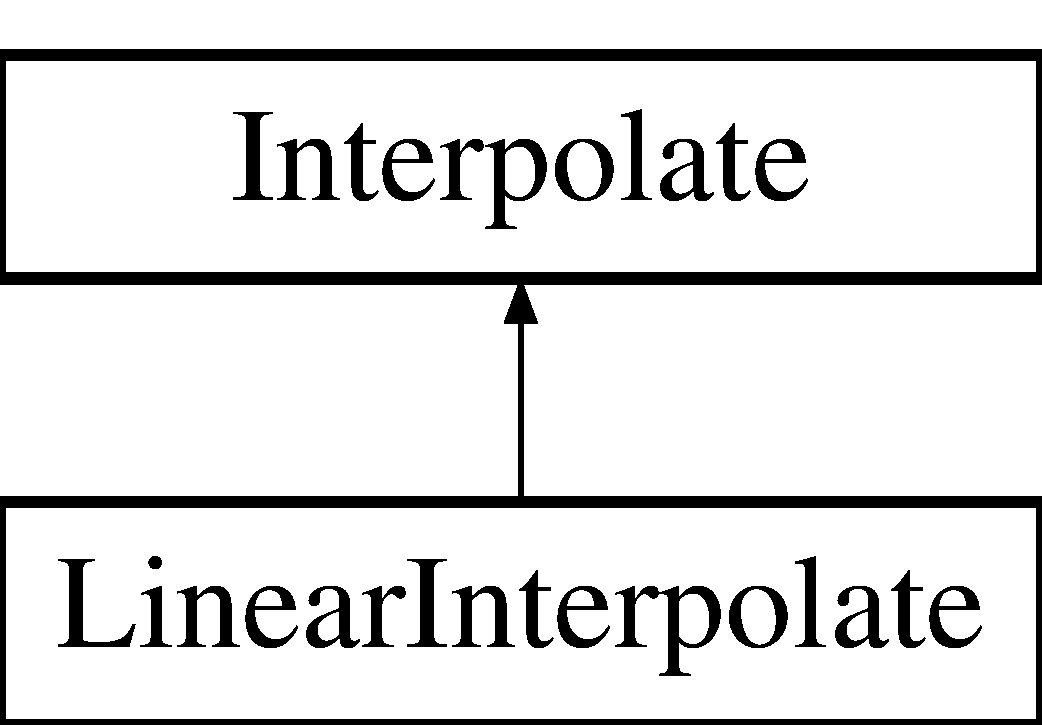
\includegraphics[height=2.000000cm]{classInterpolate}
\end{center}
\end{figure}
\subsection*{\-Public \-Member \-Functions}
\begin{DoxyCompactItemize}
\item 
\hypertarget{classInterpolate_a4525154d6de167606c69399e112a113a}{\hyperlink{classInterpolate_a4525154d6de167606c69399e112a113a}{\-Interpolate} ()}\label{classInterpolate_a4525154d6de167606c69399e112a113a}

\begin{DoxyCompactList}\small\item\em $>$ default constructor \end{DoxyCompactList}\item 
\hypertarget{classInterpolate_ae68a7e6180f1a62209d6947e2d864057}{virtual \hyperlink{classInterpolate_ae68a7e6180f1a62209d6947e2d864057}{$\sim$\-Interpolate} ()}\label{classInterpolate_ae68a7e6180f1a62209d6947e2d864057}

\begin{DoxyCompactList}\small\item\em $>$ destructor \end{DoxyCompactList}\item 
virtual bool \hyperlink{classInterpolate_af899b3717d017a8e2054e411f5f780a9}{interpolate} (\hyperlink{classGridLayer}{\-Grid\-Layer} \&gl, vector$<$ vector$<$ vector$<$ long long $>$ $>$ $>$ \&value\-Set, \hyperlink{structDataInfo}{\-Data\-Info} \&datainfo, \hyperlink{structGeometricInfo}{\-Geometric\-Info} \&geometricinfo, int interval\-Index)=0
\begin{DoxyCompactList}\small\item\em this is pure virtual function, implement how the grid\-Layer are intepolated \end{DoxyCompactList}\end{DoxyCompactItemize}


\subsection{\-Detailed \-Description}
this virtual class defines basic interface used by interpolating data in \char`\"{}grid\-Layer\char`\"{} 

this is a \char`\"{}functional\char`\"{} class, so only function supplied 

\subsection{\-Member \-Function \-Documentation}
\hypertarget{classInterpolate_af899b3717d017a8e2054e411f5f780a9}{\index{\-Interpolate@{\-Interpolate}!interpolate@{interpolate}}
\index{interpolate@{interpolate}!Interpolate@{\-Interpolate}}
\subsubsection[{interpolate}]{\setlength{\rightskip}{0pt plus 5cm}virtual bool {\bf \-Interpolate\-::interpolate} (
\begin{DoxyParamCaption}
\item[{{\bf \-Grid\-Layer} \&}]{gl, }
\item[{vector$<$ vector$<$ vector$<$ long long $>$ $>$ $>$ \&}]{value\-Set, }
\item[{{\bf \-Data\-Info} \&}]{datainfo, }
\item[{{\bf \-Geometric\-Info} \&}]{geometricinfo, }
\item[{int}]{interval\-Index}
\end{DoxyParamCaption}
)\hspace{0.3cm}{\ttfamily  \mbox{[}pure virtual\mbox{]}}}}\label{classInterpolate_af899b3717d017a8e2054e411f5f780a9}


this is pure virtual function, implement how the grid\-Layer are intepolated 


\begin{DoxyParams}{\-Parameters}
{\em gl.} & gl denote the grid\-Layer we are going to interpolating \\
\hline
{\em value\-Set.} & value\-Set will store the interpolated result \\
\hline
{\em interval\-Index.} & interval\-Index denote the interval we are going to interpolating, start from 0(included) to gl.\-size()-\/2(included) \\
\hline
\end{DoxyParams}
\begin{DoxyReturn}{\-Returns}
true means interpolate successfully, false means failed 
\end{DoxyReturn}


\-Implemented in \hyperlink{classLinearInterpolate_a1fbd904450c76999f393649026dfbd7f}{\-Linear\-Interpolate}.



\-The documentation for this class was generated from the following file\-:\begin{DoxyCompactItemize}
\item 
include/\hyperlink{Interpolate_8h}{\-Interpolate.\-h}\end{DoxyCompactItemize}

\hypertarget{classLinearInterpolate}{\section{\-Linear\-Interpolate \-Class \-Reference}
\label{classLinearInterpolate}\index{\-Linear\-Interpolate@{\-Linear\-Interpolate}}
}


\hyperlink{classLinearInterpolate}{\-Linear\-Interpolate} is used to interpolate \hyperlink{classGridLayer}{\-Grid\-Layer} linearly.  




{\ttfamily \#include $<$\-Linear\-Interpolate.\-h$>$}

\-Inheritance diagram for \-Linear\-Interpolate\-:\begin{figure}[H]
\begin{center}
\leavevmode
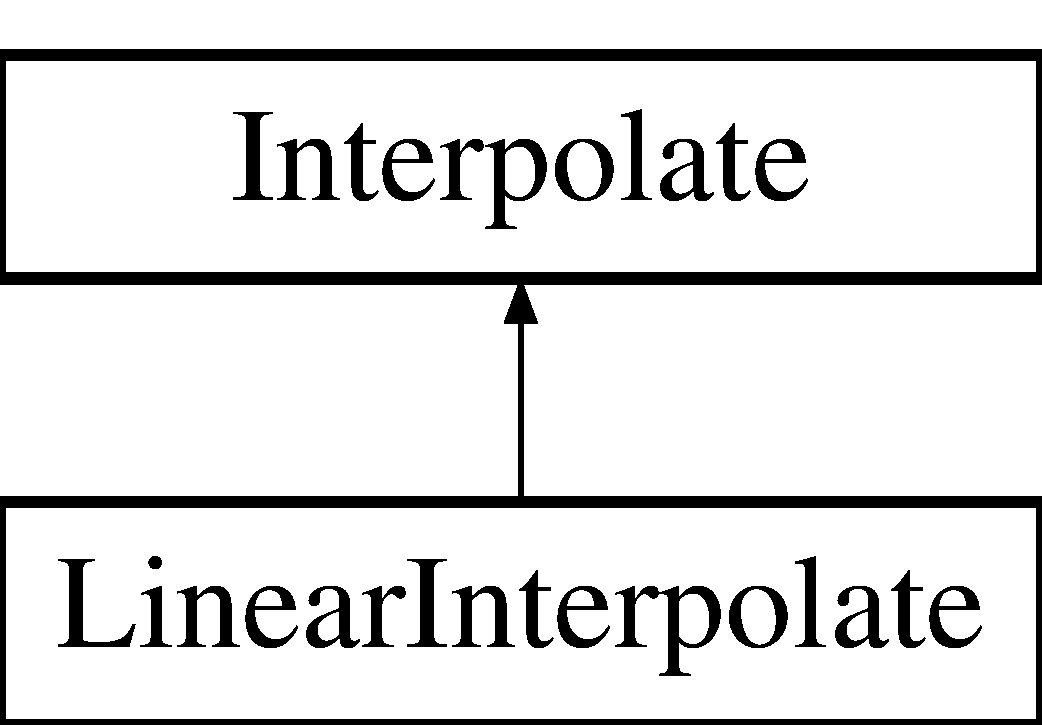
\includegraphics[height=2.000000cm]{classLinearInterpolate}
\end{center}
\end{figure}
\subsection*{\-Public \-Member \-Functions}
\begin{DoxyCompactItemize}
\item 
\hypertarget{classLinearInterpolate_a4a9fc4c8716102768917160b45f72aa1}{\hyperlink{classLinearInterpolate_a4a9fc4c8716102768917160b45f72aa1}{\-Linear\-Interpolate} ()}\label{classLinearInterpolate_a4a9fc4c8716102768917160b45f72aa1}

\begin{DoxyCompactList}\small\item\em $>$ default constructor \end{DoxyCompactList}\item 
\hypertarget{classLinearInterpolate_a1d356429366039d290d822268121a605}{\hyperlink{classLinearInterpolate_a1d356429366039d290d822268121a605}{$\sim$\-Linear\-Interpolate} ()}\label{classLinearInterpolate_a1d356429366039d290d822268121a605}

\begin{DoxyCompactList}\small\item\em $>$ destructor \end{DoxyCompactList}\item 
bool \hyperlink{classLinearInterpolate_a1fbd904450c76999f393649026dfbd7f}{interpolate} (\hyperlink{classGridLayer}{\-Grid\-Layer} \&gl, vector$<$ vector$<$ vector$<$ long long $>$ $>$ $>$ \&value\-Set, \hyperlink{structDataInfo}{\-Data\-Info} \&datainfo, \hyperlink{structGeometricInfo}{\-Geometric\-Info} \&geometricinfo, int interval\-Index)
\begin{DoxyCompactList}\small\item\em this is pure virtual function, implement how the grid\-Layer are intepolated \end{DoxyCompactList}\item 
\hypertarget{classLinearInterpolate_ae390e31d42da1e6c8658df3cb0c9c85b}{int \hyperlink{classLinearInterpolate_ae390e31d42da1e6c8658df3cb0c9c85b}{euclidean\-Algo} (int first, int second)}\label{classLinearInterpolate_ae390e31d42da1e6c8658df3cb0c9c85b}

\begin{DoxyCompactList}\small\item\em $>$ this function implement \char`\"{}\-Euclidean Algorithm\char`\"{} to calculate the greatest common divisor between \char`\"{}first\char`\"{} and \char`\"{}second\char`\"{}. \char`\"{}first\char`\"{} and \char`\"{}second\char`\"{} should be positive integer. return greatest common divisor if successfull, otherwise return -\/1. \end{DoxyCompactList}\end{DoxyCompactItemize}


\subsection{\-Detailed \-Description}
\hyperlink{classLinearInterpolate}{\-Linear\-Interpolate} is used to interpolate \hyperlink{classGridLayer}{\-Grid\-Layer} linearly. 

\-This class inherit from \char`\"{}\-Interpolate\char`\"{}, implement pure virtual function \char`\"{}interpolate\char`\"{} 

\subsection{\-Member \-Function \-Documentation}
\hypertarget{classLinearInterpolate_a1fbd904450c76999f393649026dfbd7f}{\index{\-Linear\-Interpolate@{\-Linear\-Interpolate}!interpolate@{interpolate}}
\index{interpolate@{interpolate}!LinearInterpolate@{\-Linear\-Interpolate}}
\subsubsection[{interpolate}]{\setlength{\rightskip}{0pt plus 5cm}bool {\bf \-Linear\-Interpolate\-::interpolate} (
\begin{DoxyParamCaption}
\item[{{\bf \-Grid\-Layer} \&}]{gl, }
\item[{vector$<$ vector$<$ vector$<$ long long $>$ $>$ $>$ \&}]{value\-Set, }
\item[{{\bf \-Data\-Info} \&}]{datainfo, }
\item[{{\bf \-Geometric\-Info} \&}]{geometricinfo, }
\item[{int}]{interval\-Index}
\end{DoxyParamCaption}
)\hspace{0.3cm}{\ttfamily  \mbox{[}virtual\mbox{]}}}}\label{classLinearInterpolate_a1fbd904450c76999f393649026dfbd7f}


this is pure virtual function, implement how the grid\-Layer are intepolated 


\begin{DoxyParams}{\-Parameters}
{\em gl.} & gl denote the grid\-Layer we are going to interpolating \\
\hline
{\em value\-Set.} & value\-Set will store the interpolated result \\
\hline
{\em interval\-Index.} & interval\-Index denote the interval we are going to interpolating, start from 0(included) to gl.\-size()-\/2(included) \\
\hline
\end{DoxyParams}
\begin{DoxyReturn}{\-Returns}
true means interpolate successfully, false means failed 
\end{DoxyReturn}


\-Implements \hyperlink{classInterpolate_af899b3717d017a8e2054e411f5f780a9}{\-Interpolate}.



\-The documentation for this class was generated from the following files\-:\begin{DoxyCompactItemize}
\item 
include/\hyperlink{LinearInterpolate_8h}{\-Linear\-Interpolate.\-h}\item 
src/\-Linear\-Interpolate.\-cpp\end{DoxyCompactItemize}

\hypertarget{classVolume}{\section{\-Volume \-Class \-Reference}
\label{classVolume}\index{\-Volume@{\-Volume}}
}


class \char`\"{}\-Volume\char`\"{} declare basic information for infarctate volume  




{\ttfamily \#include $<$\-Volume.\-h$>$}

\subsection*{\-Public \-Member \-Functions}
\begin{DoxyCompactItemize}
\item 
\hypertarget{classVolume_a7d3bb81da95df85009b9f3ddd985cd9f}{\hyperlink{classVolume_a7d3bb81da95df85009b9f3ddd985cd9f}{\-Volume} ()}\label{classVolume_a7d3bb81da95df85009b9f3ddd985cd9f}

\begin{DoxyCompactList}\small\item\em $>$ default constructor \end{DoxyCompactList}\item 
\hypertarget{classVolume_af048d0fefdd99ea5da2884cc05184f1c}{\hyperlink{classVolume_af048d0fefdd99ea5da2884cc05184f1c}{\-Volume} (long long \-\_\-value, int \-\_\-multiplier)}\label{classVolume_af048d0fefdd99ea5da2884cc05184f1c}

\begin{DoxyCompactList}\small\item\em $>$ overloaded constructor \end{DoxyCompactList}\item 
\hypertarget{classVolume_a050797870896c974456aace591085fcb}{\hyperlink{classVolume_a050797870896c974456aace591085fcb}{\-Volume} (const \hyperlink{classVolume}{\-Volume} \&v)}\label{classVolume_a050797870896c974456aace591085fcb}

\begin{DoxyCompactList}\small\item\em $>$ overloaded constructor \end{DoxyCompactList}\item 
\hypertarget{classVolume_a4252526a9e620590d6b08a4e88bb1226}{{\bfseries \-Volume} (vector$<$ vector$<$ \hyperlink{classBlock}{\-Block} $>$ $>$ \&s)}\label{classVolume_a4252526a9e620590d6b08a4e88bb1226}

\item 
\hypertarget{classVolume_ad5d2015f5c0fea005f02be8f6d60b212}{\hyperlink{classVolume_ad5d2015f5c0fea005f02be8f6d60b212}{$\sim$\-Volume} ()}\label{classVolume_ad5d2015f5c0fea005f02be8f6d60b212}

\begin{DoxyCompactList}\small\item\em $>$ destructor \end{DoxyCompactList}\item 
\hypertarget{classVolume_ab975dcd838fe314b403551e6d57b629c}{long long \hyperlink{classVolume_ab975dcd838fe314b403551e6d57b629c}{get\-Value} ()}\label{classVolume_ab975dcd838fe314b403551e6d57b629c}

\begin{DoxyCompactList}\small\item\em $>$ get the value of the volume \end{DoxyCompactList}\item 
\hypertarget{classVolume_a8b8d68898c25aa27b7fcc00cb57ede88}{int \hyperlink{classVolume_a8b8d68898c25aa27b7fcc00cb57ede88}{get\-Multiplier} ()}\label{classVolume_a8b8d68898c25aa27b7fcc00cb57ede88}

\begin{DoxyCompactList}\small\item\em $>$ get the multiplier used by \char`\"{}value\char`\"{} \end{DoxyCompactList}\item 
\hypertarget{classVolume_a69e856c2247a5bc28d322521699be8c6}{int \hyperlink{classVolume_a69e856c2247a5bc28d322521699be8c6}{get\-Num\-Of\-Planes} ()}\label{classVolume_a69e856c2247a5bc28d322521699be8c6}

\begin{DoxyCompactList}\small\item\em $>$ get the number of rows of the volume \end{DoxyCompactList}\item 
\hypertarget{classVolume_a8cc7673654c77b05b2fa102716ee265b}{vector$<$ \hyperlink{classBlock}{\-Block} $>$ \hyperlink{classVolume_a8cc7673654c77b05b2fa102716ee265b}{get\-Specific\-Plane} (int index)}\label{classVolume_a8cc7673654c77b05b2fa102716ee265b}

\begin{DoxyCompactList}\small\item\em $>$ get specific row. all blocks in this row line up, they stands vertically \end{DoxyCompactList}\item 
\hypertarget{classVolume_a573e89b2f9314b7dda60107420c7700c}{void \hyperlink{classVolume_a573e89b2f9314b7dda60107420c7700c}{set\-Value} (long long \-\_\-value)}\label{classVolume_a573e89b2f9314b7dda60107420c7700c}

\begin{DoxyCompactList}\small\item\em $>$ set teh value for this volume \end{DoxyCompactList}\item 
\hypertarget{classVolume_ae0bbefbd2ec7c441b4591e3dac19811d}{void \hyperlink{classVolume_ae0bbefbd2ec7c441b4591e3dac19811d}{set\-Multiplier} (int \-\_\-multiplier)}\label{classVolume_ae0bbefbd2ec7c441b4591e3dac19811d}

\begin{DoxyCompactList}\small\item\em $>$ set the multiplier used by \char`\"{}value\char`\"{} \end{DoxyCompactList}\item 
\hypertarget{classVolume_aa235c4a97c27a591efc8ccb92401e557}{bool \hyperlink{classVolume_aa235c4a97c27a591efc8ccb92401e557}{set\-Specific\-Plane} (const vector$<$ \hyperlink{classBlock}{\-Block} $>$ \&argu, int index)}\label{classVolume_aa235c4a97c27a591efc8ccb92401e557}

\begin{DoxyCompactList}\small\item\em $>$ set specific row of \-Blocks \end{DoxyCompactList}\item 
\hyperlink{classCuboid}{\-Cuboid} \hyperlink{classVolume_a8207a496fa3c9fdbdc31589659886c7b}{get\-Bounding\-Cuboid} ()
\begin{DoxyCompactList}\small\item\em $>$ get the bounding cuboid of this volume \end{DoxyCompactList}\item 
double \hyperlink{classVolume_acdc52768ad67623cb33b2de02242c9f2}{get\-Real\-Volume\-Size} (const \-Metric \&metric)
\begin{DoxyCompactList}\small\item\em $>$ get the occupied 3\-D space of the volume, parameter metric designate the metric used, can be \char`\"{}\-M\-E\-T\-E\-R\char`\"{} or \char`\"{}\-K\-I\-L\-O\-M\-E\-T\-E\-R\char`\"{} etc \end{DoxyCompactList}\item 
double \hyperlink{classVolume_afa1984fe31ad7f5c5e0a261b01bb1d2a}{get\-Real\-Shell\-Area\-Size} (const \-Metric \&metric)
\begin{DoxyCompactList}\small\item\em $>$ get the shell area of the volume, paramter metric designate the metric used, can be \char`\"{}\-M\-E\-T\-E\-R\char`\"{} or \char`\"{}\-K\-I\-L\-O\-M\-E\-T\-E\-R\char`\"{} etc \end{DoxyCompactList}\end{DoxyCompactItemize}


\subsection{\-Detailed \-Description}
class \char`\"{}\-Volume\char`\"{} declare basic information for infarctate volume 

class \char`\"{}\-Volume\char`\"{} consists of many \char`\"{}\-Block\char`\"{}s, these \char`\"{}\-Block\char`\"{}s are stored in a specific order for saving of space and analysing time. 

\subsection{\-Member \-Function \-Documentation}
\hypertarget{classVolume_a8207a496fa3c9fdbdc31589659886c7b}{\index{\-Volume@{\-Volume}!get\-Bounding\-Cuboid@{get\-Bounding\-Cuboid}}
\index{get\-Bounding\-Cuboid@{get\-Bounding\-Cuboid}!Volume@{\-Volume}}
\subsubsection[{get\-Bounding\-Cuboid}]{\setlength{\rightskip}{0pt plus 5cm}{\bf \-Cuboid} {\bf \-Volume\-::get\-Bounding\-Cuboid} (
\begin{DoxyParamCaption}
{}
\end{DoxyParamCaption}
)}}\label{classVolume_a8207a496fa3c9fdbdc31589659886c7b}


$>$ get the bounding cuboid of this volume 

$>$ haven't been finished \hypertarget{classVolume_afa1984fe31ad7f5c5e0a261b01bb1d2a}{\index{\-Volume@{\-Volume}!get\-Real\-Shell\-Area\-Size@{get\-Real\-Shell\-Area\-Size}}
\index{get\-Real\-Shell\-Area\-Size@{get\-Real\-Shell\-Area\-Size}!Volume@{\-Volume}}
\subsubsection[{get\-Real\-Shell\-Area\-Size}]{\setlength{\rightskip}{0pt plus 5cm}double {\bf \-Volume\-::get\-Real\-Shell\-Area\-Size} (
\begin{DoxyParamCaption}
\item[{const \-Metric \&}]{metric}
\end{DoxyParamCaption}
)}}\label{classVolume_afa1984fe31ad7f5c5e0a261b01bb1d2a}


$>$ get the shell area of the volume, paramter metric designate the metric used, can be \char`\"{}\-M\-E\-T\-E\-R\char`\"{} or \char`\"{}\-K\-I\-L\-O\-M\-E\-T\-E\-R\char`\"{} etc 

$>$ haven't been finished \hypertarget{classVolume_acdc52768ad67623cb33b2de02242c9f2}{\index{\-Volume@{\-Volume}!get\-Real\-Volume\-Size@{get\-Real\-Volume\-Size}}
\index{get\-Real\-Volume\-Size@{get\-Real\-Volume\-Size}!Volume@{\-Volume}}
\subsubsection[{get\-Real\-Volume\-Size}]{\setlength{\rightskip}{0pt plus 5cm}double {\bf \-Volume\-::get\-Real\-Volume\-Size} (
\begin{DoxyParamCaption}
\item[{const \-Metric \&}]{metric}
\end{DoxyParamCaption}
)}}\label{classVolume_acdc52768ad67623cb33b2de02242c9f2}


$>$ get the occupied 3\-D space of the volume, parameter metric designate the metric used, can be \char`\"{}\-M\-E\-T\-E\-R\char`\"{} or \char`\"{}\-K\-I\-L\-O\-M\-E\-T\-E\-R\char`\"{} etc 

$>$ haven't been finished 

\-The documentation for this class was generated from the following files\-:\begin{DoxyCompactItemize}
\item 
include/\hyperlink{Volume_8h}{\-Volume.\-h}\item 
src/\-Volume.\-cpp\end{DoxyCompactItemize}

\chapter{\-File \-Documentation}
\hypertarget{ArcInfoASCIIGenerator_8h}{\section{include/\-Arc\-Info\-A\-S\-C\-I\-I\-Generator.h \-File \-Reference}
\label{ArcInfoASCIIGenerator_8h}\index{include/\-Arc\-Info\-A\-S\-C\-I\-I\-Generator.\-h@{include/\-Arc\-Info\-A\-S\-C\-I\-I\-Generator.\-h}}
}


contains only one class \char`\"{}\-Arc\-Info\-A\-S\-C\-I\-I\-Generator\char`\"{}, a subclass inherit from \char`\"{}\-Data\-Generator\char`\"{}  


{\ttfamily \#include \char`\"{}\-Data\-Generator.\-h\char`\"{}}\*
\subsection*{\-Classes}
\begin{DoxyCompactItemize}
\item 
class \hyperlink{classArcInfoASCIIGenerator}{\-Arc\-Info\-A\-S\-C\-I\-I\-Generator}
\begin{DoxyCompactList}\small\item\em \hyperlink{classArcInfoASCIIGenerator}{\-Arc\-Info\-A\-S\-C\-I\-I\-Generator} is inherited from \hyperlink{classDataGenerator}{\-Data\-Generator}, responsible for generating \-A\-R\-C/\-I\-N\-F\-O \-A\-S\-C\-I\-I data file. \end{DoxyCompactList}\item 
struct \hyperlink{structArcInfoASCIIGenerator_1_1FileHeader}{\-Arc\-Info\-A\-S\-C\-I\-I\-Generator\-::\-File\-Header}
\begin{DoxyCompactList}\small\item\em file header for \-Arc/\-Info \-A\-S\-C\-I\-I file format \end{DoxyCompactList}\end{DoxyCompactItemize}


\subsection{\-Detailed \-Description}
contains only one class \char`\"{}\-Arc\-Info\-A\-S\-C\-I\-I\-Generator\char`\"{}, a subclass inherit from \char`\"{}\-Data\-Generator\char`\"{} \begin{DoxyAuthor}{\-Author}
\-Pengjie \-Zhang 
\end{DoxyAuthor}
\begin{DoxyDate}{\-Date}
2014/6/22 
\end{DoxyDate}

\hypertarget{ArcInfoASCIIParser_8h}{\section{include/\-Arc\-Info\-A\-S\-C\-I\-I\-Parser.h \-File \-Reference}
\label{ArcInfoASCIIParser_8h}\index{include/\-Arc\-Info\-A\-S\-C\-I\-I\-Parser.\-h@{include/\-Arc\-Info\-A\-S\-C\-I\-I\-Parser.\-h}}
}


this file only contains one subclass \hyperlink{classArcInfoASCIIParser}{\-Arc\-Info\-A\-S\-C\-I\-I\-Parser}, which is inherited from class \hyperlink{classDataParser}{\-Data\-Parser}  


{\ttfamily \#include \char`\"{}\-Data\-Parser.\-h\char`\"{}}\*
\subsection*{\-Classes}
\begin{DoxyCompactItemize}
\item 
class \hyperlink{classArcInfoASCIIParser}{\-Arc\-Info\-A\-S\-C\-I\-I\-Parser}
\begin{DoxyCompactList}\small\item\em class \hyperlink{classArcInfoASCIIParser}{\-Arc\-Info\-A\-S\-C\-I\-I\-Parser} is only used to parse \-Arc/\-Info \-A\-S\-C\-I\-I data file \end{DoxyCompactList}\end{DoxyCompactItemize}


\subsection{\-Detailed \-Description}
this file only contains one subclass \hyperlink{classArcInfoASCIIParser}{\-Arc\-Info\-A\-S\-C\-I\-I\-Parser}, which is inherited from class \hyperlink{classDataParser}{\-Data\-Parser} \begin{DoxyAuthor}{\-Author}
\-Pengjie \-Zhang 
\end{DoxyAuthor}
\begin{DoxyDate}{\-Date}
2014/6/23 
\end{DoxyDate}

\hypertarget{Block_8h}{\section{include/\-Block.h \-File \-Reference}
\label{Block_8h}\index{include/\-Block.\-h@{include/\-Block.\-h}}
}
{\ttfamily \#include \char`\"{}\-Metric.\-h\char`\"{}}\*
{\ttfamily \#include \char`\"{}\-Cuboid.\-h\char`\"{}}\*
\subsection*{\-Classes}
\begin{DoxyCompactItemize}
\item 
class \hyperlink{classBlock}{\-Block}
\begin{DoxyCompactList}\small\item\em class \char`\"{}\-Block\char`\"{} is specific for our project \end{DoxyCompactList}\end{DoxyCompactItemize}


\subsection{\-Detailed \-Description}
contains the definition of the class \char`\"{}\-Block\char`\"{} \begin{DoxyAuthor}{\-Author}
\-Pengjie \-Zhang 
\end{DoxyAuthor}
\begin{DoxyDate}{\-Date}
2014-\/6-\/30 
\end{DoxyDate}

\hypertarget{DataGenerator_8h}{\section{include/\-Data\-Generator.h \-File \-Reference}
\label{DataGenerator_8h}\index{include/\-Data\-Generator.\-h@{include/\-Data\-Generator.\-h}}
}


describe virtual data generator class  


{\ttfamily \#include \char`\"{}\-File\-Type.\-h\char`\"{}}\*
{\ttfamily \#include $<$string$>$}\*
\subsection*{\-Classes}
\begin{DoxyCompactItemize}
\item 
class \hyperlink{classDataGenerator}{\-Data\-Generator}
\begin{DoxyCompactList}\small\item\em virtual class to define general properties for data generator \end{DoxyCompactList}\end{DoxyCompactItemize}


\subsection{\-Detailed \-Description}
describe virtual data generator class \-This file only contains one virtual class \char`\"{}\-Data\-Generator\char`\"{}, this class provides a pure virtual function for subclass to inherit-\/-\/generate(...), subclass should be responsible to fill the actual procedure to generate corresponding data file. besides member function \char`\"{}generate(...)\char`\"{}, this class also allow users to set the resulting directory, file name for generated file.

\begin{DoxyAuthor}{\-Author}
\-Pengjie \-Zhang 
\end{DoxyAuthor}
\begin{DoxyDate}{\-Date}
2014-\/6-\/18 
\end{DoxyDate}

\hypertarget{DataParser_8h}{\section{include/\-Data\-Parser.h \-File \-Reference}
\label{DataParser_8h}\index{include/\-Data\-Parser.\-h@{include/\-Data\-Parser.\-h}}
}


this file only contains one virtual class \char`\"{}\-Data\-Parser\char`\"{}  


{\ttfamily \#include \char`\"{}\-Data\-Generator.\-h\char`\"{}}\*
{\ttfamily \#include \char`\"{}\-Grid\-Layer.\-h\char`\"{}}\*
\subsection*{\-Classes}
\begin{DoxyCompactItemize}
\item 
class \hyperlink{classDataParser}{\-Data\-Parser}
\begin{DoxyCompactList}\small\item\em virtual class \hyperlink{classDataParser}{\-Data\-Parser} is used to parse various data file format, extracting corresponding data into grid layer \end{DoxyCompactList}\end{DoxyCompactItemize}


\subsection{\-Detailed \-Description}
this file only contains one virtual class \char`\"{}\-Data\-Parser\char`\"{} \begin{DoxyAuthor}{\-Author}
\-Pengjie \-Zhang 
\end{DoxyAuthor}
\begin{DoxyDate}{\-Date}
2014/6/23 
\end{DoxyDate}

\hypertarget{FileType_8h}{\section{include/\-File\-Type.h \-File \-Reference}
\label{FileType_8h}\index{include/\-File\-Type.\-h@{include/\-File\-Type.\-h}}
}


\-This file declares what kind of file formats are supported by our project.  


\subsection*{\-Enumerations}
\begin{DoxyCompactItemize}
\item 
enum \hyperlink{FileType_8h_a2c794c5c13ab4dd7e65bad031dbe41c3}{\-File\-Type} \{ \hyperlink{FileType_8h_a2c794c5c13ab4dd7e65bad031dbe41c3aebfa06ce72c47d72d5ee9bcd73665f48}{\-N\-O\-N\-S\-E\-N\-S\-E}, 
\hyperlink{FileType_8h_a2c794c5c13ab4dd7e65bad031dbe41c3a247d522b13c8d402b516d11225da62e1}{\-A\-R\-C\-I\-N\-F\-O\-A\-S\-C\-I\-I}
 \}
\begin{DoxyCompactList}\small\item\em enum structure declares file format \end{DoxyCompactList}\end{DoxyCompactItemize}


\subsection{\-Detailed \-Description}
\-This file declares what kind of file formats are supported by our project. \-This file only contains a enum structure, all supported file formats should be registered in this structure, currently we only support \-A\-S\-C\-I\-I file format, either in text version or binary version. \begin{DoxyAuthor}{\-Author}
\-Pengjie \-Zhang 
\end{DoxyAuthor}
\begin{DoxyDate}{\-Date}
2014/6/22 
\end{DoxyDate}


\subsection{\-Enumeration \-Type \-Documentation}
\hypertarget{FileType_8h_a2c794c5c13ab4dd7e65bad031dbe41c3}{\index{\-File\-Type.\-h@{\-File\-Type.\-h}!\-File\-Type@{\-File\-Type}}
\index{\-File\-Type@{\-File\-Type}!FileType.h@{\-File\-Type.\-h}}
\subsubsection[{\-File\-Type}]{\setlength{\rightskip}{0pt plus 5cm}enum {\bf \-File\-Type}}}\label{FileType_8h_a2c794c5c13ab4dd7e65bad031dbe41c3}


enum structure declares file format 

all file formart should in uppercase word, there is a \char`\"{}null\char`\"{} file format, whenever users want to generate a data file , if the file format is \char`\"{}null\char`\"{}, stop \begin{Desc}
\item[\-Enumerator\-: ]\par
\begin{description}
\index{\-N\-O\-N\-S\-E\-N\-S\-E@{\-N\-O\-N\-S\-E\-N\-S\-E}!\-File\-Type.\-h@{\-File\-Type.\-h}}\index{\-File\-Type.\-h@{\-File\-Type.\-h}!\-N\-O\-N\-S\-E\-N\-S\-E@{\-N\-O\-N\-S\-E\-N\-S\-E}}\item[{\em 
\hypertarget{FileType_8h_a2c794c5c13ab4dd7e65bad031dbe41c3aebfa06ce72c47d72d5ee9bcd73665f48}{\-N\-O\-N\-S\-E\-N\-S\-E}\label{FileType_8h_a2c794c5c13ab4dd7e65bad031dbe41c3aebfa06ce72c47d72d5ee9bcd73665f48}
}]as word denotes, this file format is nonsense, used in situation in which no file format is used. \index{\-A\-R\-C\-I\-N\-F\-O\-A\-S\-C\-I\-I@{\-A\-R\-C\-I\-N\-F\-O\-A\-S\-C\-I\-I}!\-File\-Type.\-h@{\-File\-Type.\-h}}\index{\-File\-Type.\-h@{\-File\-Type.\-h}!\-A\-R\-C\-I\-N\-F\-O\-A\-S\-C\-I\-I@{\-A\-R\-C\-I\-N\-F\-O\-A\-S\-C\-I\-I}}\item[{\em 
\hypertarget{FileType_8h_a2c794c5c13ab4dd7e65bad031dbe41c3a247d522b13c8d402b516d11225da62e1}{\-A\-R\-C\-I\-N\-F\-O\-A\-S\-C\-I\-I}\label{FileType_8h_a2c794c5c13ab4dd7e65bad031dbe41c3a247d522b13c8d402b516d11225da62e1}
}]denote standard \-A\-R\-C/\-I\-N\-F\-O \-A\-S\-C\-I\-I file format \end{description}
\end{Desc}


\hypertarget{GenerateBlock_8h}{\section{include/\-Generate\-Block.h \-File \-Reference}
\label{GenerateBlock_8h}\index{include/\-Generate\-Block.\-h@{include/\-Generate\-Block.\-h}}
}
{\ttfamily \#include \char`\"{}\-Interpolate.\-h\char`\"{}}\*
{\ttfamily \#include \char`\"{}\-Block.\-h\char`\"{}}\*
{\ttfamily \#include \char`\"{}\-Grid\-Layer.\-h\char`\"{}}\*
\subsection*{\-Classes}
\begin{DoxyCompactItemize}
\item 
class \hyperlink{classGenerateBlock}{\-Generate\-Block}
\begin{DoxyCompactList}\small\item\em class \hyperlink{classGenerateBlock}{\-Generate\-Block} is used to generate \-Blocks from interpolated \hyperlink{classGridLayer}{\-Grid\-Layer} \end{DoxyCompactList}\end{DoxyCompactItemize}


\subsection{\-Detailed \-Description}
contains the class used to generate block from \hyperlink{classGridLayer}{\-Grid\-Layer} \begin{DoxyAuthor}{\-Author}
\-Pengjie \-Zhang 
\end{DoxyAuthor}
\begin{DoxyDate}{\-Date}
2014-\/7-\/23 
\end{DoxyDate}

\hypertarget{GenerateVolume_8h}{\section{include/\-Generate\-Volume.h \-File \-Reference}
\label{GenerateVolume_8h}\index{include/\-Generate\-Volume.\-h@{include/\-Generate\-Volume.\-h}}
}
{\ttfamily \#include \char`\"{}\-Block.\-h\char`\"{}}\*
{\ttfamily \#include \char`\"{}\-Grid\-Layer.\-h\char`\"{}}\*
{\ttfamily \#include \char`\"{}\-Interpolate.\-h\char`\"{}}\*
{\ttfamily \#include \char`\"{}\-Volume.\-h\char`\"{}}\*
\subsection*{\-Classes}
\begin{DoxyCompactItemize}
\item 
class \hyperlink{classGenerateVolume}{\-Generate\-Volume}
\begin{DoxyCompactList}\small\item\em this class is used to generate volumes \end{DoxyCompactList}\end{DoxyCompactItemize}


\subsection{\-Detailed \-Description}
contains the declaration of data sturctures used to generate volumes \begin{DoxyAuthor}{\-Author}
\-Pengjie \-Zhang 
\end{DoxyAuthor}
\begin{DoxyDate}{\-Date}
2014-\/7-\/23 
\end{DoxyDate}

\hypertarget{GridLayer_8h}{\section{include/\-Grid\-Layer.h \-File \-Reference}
\label{GridLayer_8h}\index{include/\-Grid\-Layer.\-h@{include/\-Grid\-Layer.\-h}}
}


\-This file contains one class and several auxiliary data structure.  


{\ttfamily \#include $<$vector$>$}\*
{\ttfamily \#include $<$stdlib.\-h$>$}\*
{\ttfamily \#include $<$iostream$>$}\*
{\ttfamily \#include \char`\"{}\-File\-Type.\-h\char`\"{}}\*
{\ttfamily \#include \char`\"{}\-Metric.\-h\char`\"{}}\*
\subsection*{\-Classes}
\begin{DoxyCompactItemize}
\item 
struct \hyperlink{structDataInfo}{\-Data\-Info}
\begin{DoxyCompactList}\small\item\em data structure to keep some detailed information for the data in a data file \end{DoxyCompactList}\item 
struct \hyperlink{structGeometricInfo}{\-Geometric\-Info}
\begin{DoxyCompactList}\small\item\em \hyperlink{structGeometricInfo}{\-Geometric\-Info} data structure is used to record ths geometric info about the grids in a grid layer. \end{DoxyCompactList}\item 
class \hyperlink{classGridLayer}{\-Grid\-Layer}
\begin{DoxyCompactList}\small\item\em class accept only integer value. \end{DoxyCompactList}\end{DoxyCompactItemize}


\subsection{\-Detailed \-Description}
\-This file contains one class and several auxiliary data structure. even most data file provide float value, the grid layer should only store integer for easy of analysing. \-So actually, the value type in grid layer is alwasy \char`\"{}long long int\char`\"{}, if necessary, we will try to use big\-Int library later. \-All float values in data file will be transfer to integer before storing into a gridlayer either by multiplying a multiplier then rounded or dividing by a divisor then rounded. \-For a data file, all its numeric will be under the same processing \begin{DoxyAuthor}{\-Author}
\-Pengjie \-Zhang 
\end{DoxyAuthor}
\begin{DoxyDate}{\-Date}
2014-\/7-\/23
\end{DoxyDate}
contains the definition of class \char`\"{}\-Grid\-Layer\char`\"{} \begin{DoxyAuthor}{\-Author}
\-Pengjie \-Zhang 
\end{DoxyAuthor}
\begin{DoxyDate}{\-Date}
2014-\/7-\/23 
\end{DoxyDate}

\hypertarget{Interpolate_8h}{\section{include/\-Interpolate.h \-File \-Reference}
\label{Interpolate_8h}\index{include/\-Interpolate.\-h@{include/\-Interpolate.\-h}}
}
{\ttfamily \#include \char`\"{}\-Grid\-Layer.\-h\char`\"{}}\*
{\ttfamily \#include $<$vector$>$}\*
\subsection*{\-Classes}
\begin{DoxyCompactItemize}
\item 
class \hyperlink{classInterpolate}{\-Interpolate}
\begin{DoxyCompactList}\small\item\em this virtual class defines basic interface used by interpolating data in \char`\"{}grid\-Layer\char`\"{} \end{DoxyCompactList}\end{DoxyCompactItemize}


\subsection{\-Detailed \-Description}
defines virtual class \char`\"{}\-Interpolate\char`\"{}, this class family is used to indicate how the data in \char`\"{}grid\-Layer\char`\"{} are interpolate \begin{DoxyAuthor}{\-Author}
\-Pengjie \-Zhang 
\end{DoxyAuthor}
\begin{DoxyDate}{\-Date}
2014-\/7-\/28 
\end{DoxyDate}

\hypertarget{LinearInterpolate_8h}{\section{include/\-Linear\-Interpolate.h \-File \-Reference}
\label{LinearInterpolate_8h}\index{include/\-Linear\-Interpolate.\-h@{include/\-Linear\-Interpolate.\-h}}
}
{\ttfamily \#include \char`\"{}\-Interpolate.\-h\char`\"{}}\*
\subsection*{\-Classes}
\begin{DoxyCompactItemize}
\item 
class \hyperlink{classLinearInterpolate}{\-Linear\-Interpolate}
\begin{DoxyCompactList}\small\item\em \hyperlink{classLinearInterpolate}{\-Linear\-Interpolate} is used to interpolate \hyperlink{classGridLayer}{\-Grid\-Layer} linearly. \end{DoxyCompactList}\end{DoxyCompactItemize}


\subsection{\-Detailed \-Description}
declare class \char`\"{}\-Linear\-Interpolate\char`\"{}, this class is used to linearly interpolate \hyperlink{classGridLayer}{\-Grid\-Layer} \begin{DoxyAuthor}{\-Author}
\-Pengjie \-Zhang 
\end{DoxyAuthor}
\begin{DoxyDate}{\-Date}
2014-\/7-\/28 
\end{DoxyDate}

\hypertarget{Volume_8h}{\section{include/\-Volume.h \-File \-Reference}
\label{Volume_8h}\index{include/\-Volume.\-h@{include/\-Volume.\-h}}
}
{\ttfamily \#include \char`\"{}\-Metric.\-h\char`\"{}}\*
{\ttfamily \#include \char`\"{}\-Block.\-h\char`\"{}}\*
{\ttfamily \#include $<$vector$>$}\*
\subsection*{\-Classes}
\begin{DoxyCompactItemize}
\item 
class \hyperlink{classVolume}{\-Volume}
\begin{DoxyCompactList}\small\item\em class \char`\"{}\-Volume\char`\"{} declare basic information for infarctate volume \end{DoxyCompactList}\end{DoxyCompactItemize}


\subsection{\-Detailed \-Description}
contains the declaration of class \char`\"{}\-Volume\char`\"{} \begin{DoxyAuthor}{\-Author}
\-Pengjie \-Zhang 
\end{DoxyAuthor}
\begin{DoxyDate}{\-Date}
2014-\/7-\/23 
\end{DoxyDate}

\hypertarget{Block_8cpp}{\section{src/\-Block.cpp \-File \-Reference}
\label{Block_8cpp}\index{src/\-Block.\-cpp@{src/\-Block.\-cpp}}
}
{\ttfamily \#include \char`\"{}\-Block.\-h\char`\"{}}\*


\subsection{\-Detailed \-Description}
contains the definition of the class \char`\"{}\-Block\char`\"{} \begin{DoxyAuthor}{\-Author}
\-Pengjie \-Zhang 
\end{DoxyAuthor}
\begin{DoxyDate}{\-Date}
2014-\/6-\/30 
\end{DoxyDate}

\printindex
\end{document}
